% !TeX document-id = {075bf025-0d99-414a-b21e-a2ac906020fb}
% !TeX encoding = UTF-8
% !TeX program = pdflatex
% !BIB program = biber
% Template Revision:
% Rev. A2 -- 2019-11-04 -- A. Varli
% Rev. B1 -- 2019-11-05 -- A. Varli
%% HINWEISE:
%% MAIN.tex ist die Hauptdatei. Hier sind sämtliche Pakete eingebunden und die allgemeine Struktur ist hier festgelegt. Im Allgemeinen müssen hier keine Änderungen vorgenommen werden.
%% In der eingebundenen Datei config.tex müssen Änderungen vorgenommen werden, die in der Datei näher erläutert sind.
%% Das Deckblatt wird mit der Datei cover/coversheet.tex eingebunden. Hier sollten keine Änderungen vorgenommen werden.
%% Für Text im Vorspann (vor der Inhaltsangabe, z.B. für Vorwort, Abstract etc.) ist die Datei frontmatter.tex vorgesehen.
%% Für den Hauptteil ist die Datei mainmatter.tex vorgesehen.
%% Das Literaturverzeichnis ist die eingebundene Datei literature.bib.
%% Für Verbesserungsvorschläge bin ich gerne offen.
%% Viel Erfolg :). Linz, im Oktober 2019, Ali Varli, a_v@gmx.net.
%% PLEASE NOTE:
%% MAIN.tex is the main file. All packages are pooled here and the general structure is defined here. In general, no changes need to be made here.
%% Changes must be made in the included file config.tex. Detailed information is in the file.
%% The cover page is included with the file cover/coversheet.tex. No changes should be made here.
%% The file frontmatter.tex is provided for text in the lead text (before the summary, i.e. for the foreword, abstract, etc.).
%% The file mainmatter.tex is intended for the main part.
%% The bibliography is the included file literature.bib.
%% I am open to suggestions for improvement.
%% Good luck :-). Linz, October 2019, Ali Varli, a_v@gmx.net.
\documentclass[
		a4paper,
		oneside,
		onecolumn,
		openany,
		parskip=half*,
%		toc=flat,
%		chapterentrydots=true,
		table,
		11pt,
		fleqn,
%		draft
	]{scrbook}
	
	\usepackage[utf8]{inputenc}

	% !TeX encoding = UTF-8
% !TeX root = MAIN.tex

\newif\ifeng
%% HINWEISE: Hier müssen folgende Einstellungen vorgenommen werden:
%% PLEASE NOTE: Select your settings here:

%% Sprache: Falls die Dokumentensprache Deutsch ist, \engtrue mit einem %-Zeichen davor auskommentieren:
%% Language: If the document language is German, comment \engtrue with a % sign in front:
	\engtrue
	
%% Hier den Namen des Autors eingeben:
%% Enter the author’s name here:
	\def\name{Franz Miketta}
	
%% Hier Informationen für den rechten Block unter dem JKU-Logo eingeben, wobei die Elemente mit einem Buchstaben jeweils für die Überschrift und mit Doppelbuchstaben für den Inhalt sind. Falls Elemente nicht benötigt werden, bitte NICHT LÖSCHEN, sondern frei lassen, wie z.B. elementE bzw. elementEE.  
%% Enter information here for the right block under the JKU logo, whereby the elements should have one letter for the heading and double letters for content. If the elements are not needed, DO NOT DELETE them. Simply leave them blank, such as elementE and/or elementEE.  
	\def\elementA{Submitted by}
	\def\elementAA{\textbf{\name}}

	\def\elementB{Submitted at}
	\def\elementBB{\textbf{Institute for System Software}}

	\def\elementC{Supervisor}
	\def\elementCC{\textbf{tbd}}

	\def\elementD{Co-Supervisor}
	\def\elementDD{\textbf{Dr. Christian Wirth}}

	\def\elementE{Co-Supervisor}
	\def\elementEE{\textbf{Dr. Daniele Bonetta}}

%% Hier Datum eingeben:
%% Enter the date:  
	\def\date{\today}
	
%% Hier Ort eingeben:
%% Enter the location:
	\def\place{Linz}
	
%% Hier Titel eingeben; steht über dem K:
%% Enter the title; it appears above the K:
	\def\title{Contributing the ECMAScript proposal ``Module blocks'' into Graal.js}

%% Hier ggf. Untertitel und LVA eingeben; stehen unter dem K. Falls sie nicht benötigt werden, bitte NICHT LÖSCHEN sondern frei lassen:
%% If necessary, enter a subtitle and course here; below the K. If they are not needed, please DO NOT DELETE them. Simply leave them blank.
	\def\subtitle{Contributing an ECMAScript proposal into Graal.js}
	\def\lva{Bachelor thesis}
	
%% Hier ggf. Metadaten für das PDF eingeben. Falls sie nicht benötigt werden, bitte NICHT LÖSCHEN sondern frei lassen:
%% If necessary, enter metadata for the PDF here. If it is not needed, please DO NOT DELETE them. Simply leave them blank:
	\def\pdfTitle{\title}
	\def\pdfAuthor{\name}
	\def\pdfSubject{}
	\def\pdfKeywords{}
	
\newif\ifthesis
%% Ab hier müssen nur Änderungen vorgenommen werden, falls es sich um eine Bachelor- oder Masterarbeit oder eine Dissertation handelt. Wenn es sich darum handelt, die Auskommentierung der folgenden Zeile aufheben:
%% Starting from this point on, only enter any changes if it is a Bachelor's or Master's thesis or a dissertation. If this is the case, uncomment the following line:
	\thesistrue

%% Hier den Typ der Arbeit eingeben (0: Bachelorarbeit, 1: Masterarbeit, 2: Dissertation, 3: Diplomarbeit):
%% Enter the type of paper here (0: Bachelor’s Thesis, 1: Master’s Thesis, 2: Dissertation, 3: Diploma Degree Thesis):
	\def\type{0}

%% Hier den angestrebten akademischen Grad eingeben:
%% Enter the desired academic degree here:
	\def\degree{Bachelor of Science}

%% Hier die Studienrichtung eingeben:
%% Enter the major here:
	\def\study{Informatik}

	
	\usepackage[T1]{fontenc}
	\usepackage{roboto}
	\usepackage{mathpazo}
	    
	\ifeng	\usepackage[ngerman,english]{babel}
	\else	\usepackage[english,ngerman]{babel}	
	\fi
		
	\usepackage{amsmath}
	\usepackage{siunitx}	

%% Zitierweise numerisch, Literaturverzeichnis alphabetisch sortiert:
%% Citation listed numerically, bibliography listed alphabetically:
	\usepackage[backend=biber,sortlocale=auto,style=numeric-comp]{biblatex}
%% Zitierweise numerisch, Literaturverzeichnis unsortiert:
%% Citation listed numerically, bibliography unsorted:
%	\usepackage[backend=biber,sorting=none,style=numeric-comp]{biblatex}
%% Zitierweise Autor-Jahr, Literaturverzeichnis alphabetisch sortiert:
%% Citation listed by author-year, bibliography listed alphabetically:
%	\usepackage[backend=biber,style=authoryear,bibstyle=authoryear,citestyle=authoryear,maxcitenames=2]{biblatex}
	\addbibresource{literature.bib}
    \usepackage{csquotes}
    
    \usepackage[a4paper,left=30mm,right=14mm,top=27mm,bottom=10mm,includeheadfoot]{geometry}

	\usepackage{lastpage}
	\usepackage{scrlayer-scrpage}
	\pagestyle{scrheadings}
	\clearscrheadfoot
	\ifeng	\ohead*{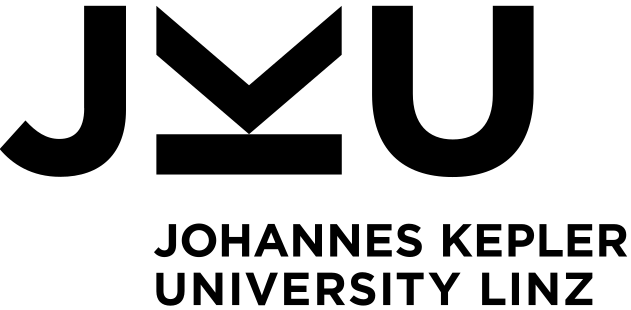
\includegraphics[width=3cm]{cover/jkuen.png}}
	\else	\ohead*{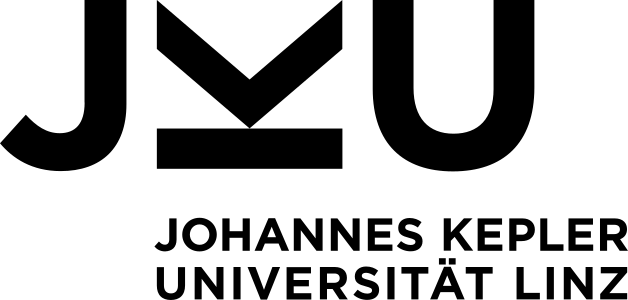
\includegraphics[width=3cm]{cover/jkude.png}}
	\fi
	\ifoot*{\date}
	\cfoot*{\name}
	\ofoot*{\pagemark/\pageref{LastPage}}	
	\setkomafont{pageheadfoot}{\sffamily \scriptsize}
	\setkomafont{pagenumber}{\sffamily \scriptsize}

	\usepackage[onehalfspacing]{setspace}
	
	\usepackage{pdfpages}

	\usepackage{tabularx}
	\usepackage{ltxtable}
	\usepackage{booktabs}
	\usepackage{rotating}
	\usepackage{colortbl}
	\usepackage{multirow}
	\usepackage{adjustbox}
	
	\usepackage{xcolor}

	\usepackage{graphicx}
	\usepackage{wrapfig}

	\usepackage[section]{placeins} %\FloatBarrier

	\usepackage{float} %[H]

	\usepackage{enumitem}
		
	\usepackage{subfiles}
	
	\usepackage{listings}
	
%	\usepackage[toc,lof,lot]{multitoc}

%	\usepackage[
%		bookmarksnumbered=true,
%		pdfborder={0 0 0},
%		pdfa,
%		pdftitle={\pdfTitle},
%		pdfauthor={\pdfAuthor},
%		pdfsubject={\pdfSubject},
%		pdfkeywords={\pdfKeywords}]{hyperref}
	
%	\setcounter{tocdepth}{3} %subsubsection
%	\setcounter{secnumdepth}{3}
		
	\tolerance=100
	\clubpenalty=10000
	\widowpenalty=10000
	\displaywidowpenalty=10000
	
%	\addtocontents{toc}{\protect\enlargethispage{2\normalbaselineskip}}
%	\addtocontents{lof}{\protect\enlargethispage{2\normalbaselineskip}}
%	\addtocontents{lot}{\protect\enlargethispage{2\normalbaselineskip}}
	
	\addtokomafont{caption}{\small}
	\setkomafont{captionlabel}{\small\sffamily\bfseries}
	
	
	% own shit
	\usepackage{color}
	\definecolor{lightgray}{rgb}{.9,.9,.9}
	\definecolor{darkgray}{rgb}{.4,.4,.4}
	\definecolor{purple}{rgb}{0.65, 0.12, 0.82}
	\definecolor{lightorange}{rgb}{1,0.63,0}
	\definecolor{lightgreen}{rgb}{0,1,0.63}
	\definecolor{lightblue}{rgb}{0.31,0.63,1}
	
	\lstdefinelanguage{JavaScript}{
		keywords={typeof, new, true, false, catch, function, return, null, catch, switch, var, if, in, while, do, else, case, break},
		keywordstyle=\color{blue}\bfseries,
		ndkeywords={class, export, boolean, throw, implements, import, this},
		ndkeywordstyle=\color{darkgray}\bfseries,
		identifierstyle=\color{black},
		sensitive=false,
		comment=[l]{//},
		morecomment=[s]{/*}{*/},
		commentstyle=\color{purple}\ttfamily,
		stringstyle=\color{red}\ttfamily,
		morestring=[b]',
		morestring=[b]"
	}
	
	\lstset{
		language=JavaScript,
		backgroundcolor=\color{lightgray},
		extendedchars=true,
		basicstyle=\footnotesize\ttfamily,
		showstringspaces=false,
		showspaces=false,
		numbers=left,
		numberstyle=\footnotesize,
		numbersep=9pt,
		tabsize=2,
		breaklines=true,
		showtabs=false,
		captionpos=b
	}

\renewcommand\lstlistingname{List of Listings}
\renewcommand\lstlistlistingname{List of Listings}

%\usepackage{tikz}
%\usetikzlibrary{positioning}
%\usetikzlibrary{graphdrawing.trees}
%
%%
%%%%
%%%%%%%%
%%%%%%%%%%%%%%%%
\begin{document}
%%%%%%%%%%%%%%%%

\begin{titlepage}
{
\singlespacing
\parindent 0pt
\def\ifundefined#1{\expandafter\ifx\csname#1\endcsname\relax}
\makeatletter
\def\Huge{\@setfontsize\Huge{28pt}{28}}
\makeatother
\unitlength 1cm
\sffamily	
\small
%
%
\begin{picture}(16.6,0)
 \ifeng
  \put(11.2,0){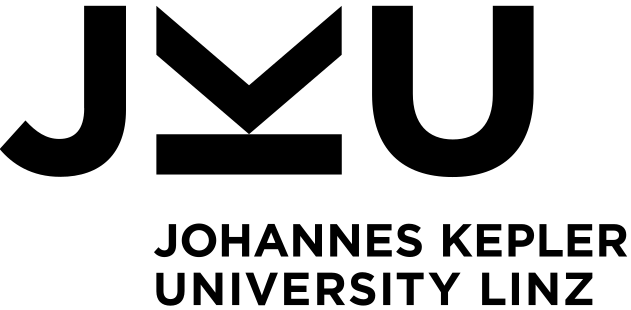
\includegraphics[width=5.2cm]{cover/jkuen}}
 \else
  \put(11.2,0){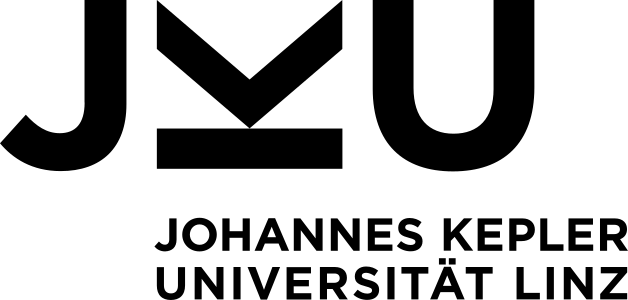
\includegraphics[width=5.2cm]{cover/jkude}}
 \fi
 \put(12.6,-1.7){%
  \begin{minipage}[t]{3.9cm}
   \begin{flushleft}
	\ifdefined\elementA
	 {\footnotesize\elementA \vskip.1mm}
	 {\elementAA}
	 \vskip5mm
	\else
	 \relax
	\fi
	\ifdefined\elementB
	 {\footnotesize\elementB \vskip.1mm}
	 {\elementBB}
	 \vskip5mm
	\else
	 \relax
	\fi
	\ifdefined\elementC
	 {\footnotesize\elementC \vskip.1mm}
	 {\elementCC}
	 \vskip5mm
	\else
	 \relax
	\fi
	\ifdefined\elementD
	 {\footnotesize\elementD \vskip.1mm}
	 {\elementDD}
	 \vskip5mm
	\else
	 \relax
	\fi
	\ifdefined\elementE
	 {\footnotesize\elementE \vskip.1mm}
	 {\elementEE}
	 \vskip5mm
	\else
	 \relax
	\fi
	\date
   \end{flushleft}
  \end{minipage}
 }
%	
%	
 \put(12.6,-21.5){%
  \begin{minipage}[t]{3.9cm}
   {\fontseries{black}\selectfont JOHANNES KEPLER\\
  \ifeng
   UNIVERSITY
  \else
   UNIVERSIT\"{A}T
  \fi
   LINZ}\\
   Altenbergerstra{\ss}e 69\\
   4040 Linz, \"{O}sterreich\\
   www.jku.at\\
   DVR 0093696
  \end{minipage}
 }
%
%		
 \put(0,-10.2){\begin{minipage}[b]{12cm}
 \fontseries{black}\selectfont
 {\begin{flushleft}
 \Huge \expandafter\MakeUppercase\expandafter \title
 \end{flushleft}} \end{minipage}}
%	
 \put(0,-15.2){
\includegraphics[width=4.4cm]{cover/arr}}
%	
 \put(0,-16.3){\begin{minipage}[t]{12cm}
  \ifthesis \Large
   \ifeng
    \ifcase\type Bachelor \or Master \or Doctoral \or Diploma \fi Thesis \vskip1mm
    {\normalsize to obtain the academic degree of} \vskip2mm
    \degree \vskip1mm
    {\normalsize in the \ifcase\type Bachelor's \or Master's \or  Doctoral \or Diploma \fi Program} \vskip2mm
   \else
    \ifcase\type Bachelorarbeit \or Masterarbeit \or Dissertation \or Diplomarbeit \fi \vskip1mm
    {\normalsize zur Erlangung des akademischen Grades} \vskip2mm
    \degree \vskip1mm
    {\normalsize im \ifcase\type Bachelorstudium \or Masterstudium \or  Doktoratsstudium \or Diplomstudium \fi} \vskip2mm
   \fi
    \study
  \else
   {\Large\lva}
   \vskip2mm
   {\Large\bfseries\subtitle} 
   \fi
 \end{minipage}}
\end{picture}
}

\end{titlepage}


%%%%%%%%%%%%
\frontmatter

% !TeX encoding = UTF-8
% !TeX root = MAIN.tex

	\ifeng \chapter*{Statutory Declaration}
	I hereby declare under oath that the submitted thesis has been written solely by me without any third-party assistance, information other than provided sources or aids have not been used and those used have been fully documented. Sources for literal, paraphrased and cited quotes have been accurately credited.
	
	The submitted document here present is identical to the electronically submitted text document.
	
	\vskip1cm
	\place, \date
	
	\else \chapter*{Eidesstattliche Erklärung}
	Ich erkläre an Eides statt, dass ich die vorliegende Arbeit selbstständig und ohne fremde Hilfe verfasst, andere als die angegebenen Quellen und Hilfsmittel nicht benutzt bzw. die wörtlich oder sinngemäß entnommenen Stellen als solche kenntlich gemacht habe.

	Die vorliegende Arbeit ist mit dem elektronisch übermittelten Textdokument identisch.
	
	\vskip1cm
	\place, \date
	\fi


	\ifeng	\chapter*{Abstract}
	\else	\chapter*{Kurzfassung}
	\fi
		
%% Hier Abstact in der Sprache eingeben, in der die Arbeit geschrieben wurde.
%% Enter here the abstract in the main language.

The thesis aims at implementing an ECMAScript proposal from the TC39 proposals, the module blocks, into the existing Graal.js interpreter. Besides the initial task of changing the parser and the runtime and unit tests, the base framework for shipping code between processes is implemented and explicit benchmarks are shown. The final product contributes to the open source version of Graal.js on the platform github.com.

	{\let\clearpage\relax
	\ifeng	\selectlanguage{ngerman} \chapter*{Zusammenfassung}
	\else	\selectlanguage{english} \chapter*{Abstract}
	\fi
		
%% Hier Abstact in der jeweils anderen Sprache eingeben.
%% Enter here the abtract in the other language.

Die vorliegende Arbeit verfolgt das Ziel einen ECMAScript-Erweiterungsvorschlag aus den TC39-Erweiterungsvorschlägen, die module blocks, im bestehenden Graal.js-Interpreter zu implementieren. Nach der Implementierung im Parser und der Runtime und entsprechenden Tests wird weiters ein Framework zum Übertragen von Code zwischen Prozessen eingerichtet und dessen Performance mit ursprünglichen Implementierungen verglichen. Die finale Implementierung wird über die Plattform github.com der Open-Source-Version von Graal.js hinzugefügt.

	\ifeng	\selectlanguage{english}
	\else 	\selectlanguage{ngerman}
	\fi}


\begin{singlespace}
\tableofcontents
\end{singlespace}
	

%%%%%%%%%%%	
\mainmatter

% !TeX encoding = UTF-8
% !TeX root = MAIN.tex

\chapter{Introduction}

The following paragraphs serve as an introduction to the thesis by explaining the relevance both for \emph{GraalVM} and \emph{Graal.js} in general and in the specific case of the ECMAScript proposal \emph{module blocks}. The last paragraph explains the outline of the thesis.

ECMAScript is the standardized version of the famous internet front-end scripting language JavaScript.  The ECMAScript specification includes language features and their expected behavior each scripting language should have. The specification then in turn is implemented by so-called engines that run JavaScript code. JavaScript is on spot three on the PYPL popularity index for programming languages indicating its popularity by google search trends. \cite{pypl} As a core technology of the internet it helped shaping the web as we see it today. An important part in the language becoming a core technology was browser support which had been a problem in the past. An issue arose for websites called interoperability across web browsers where the pages had to be programmed differently for each browser otherwise they would look divergently or even wouldn't work at all. \cite{10.1145/3386327} This issue was fixed by ECMAScript. Meanwhile a browser's engine's support is determined by feature support of the ECMAScript specification. The language specification development doesn't stagnate but is standardized via a proposal process which is divided into five stages and is overlooked by an installed ECMA-committee. Thus new language features bundled into versions are developed in a standardized environment with the web community and vendors together as a team. \cite{ecma}

In 2019 Oracle released the GraalVM with active development up to present days. GraalVM is a multilingual runtime with multiple core features such as certain compiler optimizations, ahead-of-time compilation, polyglot programming, LLVM runtime and the Truffle language implementation framework. With the amount of supported programming languages and the foregoing mentioned features the GraalVM can be implemented into a variety of production environments. One environment seems of particular interest: Microservices on server environments. The GraalVM native image was able to lower startup time and memory footprint by a significant amount. \cite{graalVMNative} These savings won over the social media platform Twitter which Microservices run on GraalVM and GraalVM in return created savings for their CPU times which makes it have an environmental impact. The other core feature of GraalVM is the support of multiple languages via the Truffle framework. With this framework different languages can be implemented on top of GraalVM. \cite{graalVMStart}\cite{graalVMIntro} The framework itself provide The different language implementations are split up into single projects for each language. This setup leads to the project Graal.js.

Graal.js is the Truffle implementation of ECMAScript on the GraalVM. The project embeds the language specification into the Truffle framework. In general the project transforms JavaScript source code into an abstract syntax tree to be executed by any Java Virtual Machine (JVM). \cite{Graaljs} The main components to be introduced for the task include a parser, nodes for the resulting abstract syntax tree and a transformation logic for translating the parser produced intermediate representation to the aforementioned abstract syntax tree. The Graal.js interpreter together with any JVM, preferably the GraalVM, is an ECMAScript engine and thus has to compete with other ECMAScript engines. With the official release of GraalVM 21 it showed to be on par with V8, Google's engine, and Spidermonkey, Mozilla's engine, with all three supporting 99\% of the newest ECMAScript version. \cite{kangax1} The big advantage Graal.js has over the other two engines is being embedded in the GraalVM ecosystem allowing polyglot programs. To keep up with current development the Graal.js project aims to implement proposal that haven't gone the whole way of the aforementioned proposal process and are yet to be released as new features of ECMAScript to be ahead of time. One of these yet to pass the process proposals is the module block proposal.

Module blocks are an effort by Daniel Ehrenberg and Surma based on inline modules. Inlining modules is a feature which is missing from the current ECMAScript. The absence has resulted into workarounds with various issues. ECMAScript cannot share code between processes thus residing on a single thread. Every module, worker and worklet needs a separate file cluttering project folders. Tasks short of stringification cannot be shared across agents. The multitude of problems cited can be addressed by module blocks. Module blocks are a stage 2 proposal on ECMAScript 262 and is most likely to be implemented in the 2022 version of ECMAScript. \cite{gitMB} Since it has a high relevance for polyglot programs its implementation is key to staying on top of the technology stack which brings us to the purpose of this thesis.

The main objective of this thesis is to implement the new ECMAScript stage 2 proposal module blocks into the Graal.js engine which is implemented via the Truffle framework. Furthermore testing for this implementation will be conducted. When the general workings are set a code shipping framework and benchmarks will be included.

The thesis is divided into five further chapters. Section two explains the theoretical background of the thesis. In the following chapter three the implementation and the testing is addressed. Afterwards Section four handles benchmarking. The thesis is then rounded up in Section five and six by highlighting future work and a conclusion.

% further notes to think about on thesis introduction
%Runtime relevancy - to stay relevant new features need to be implemented asap - module blocks\\

%module blocks -> inline modules -> general idea is to ship code between processes and thus potentially between machines over network -> bring logic to data not vice versa -> esp. important in database business environments

%Outline of thesis - 

\chapter{Background}

\emph{This chapter lays out the theoretical background of this thesis by first introducing the general concepts of a high-level language virtual machine (HLL-VM) like the Java Virtual Machine (JVM) and then going on to more specific features of the GraalVM. In the following the next abstraction layer the Truffle API is explained before coming to the explicit project Graal.js which uses Truffle. The last section evolves around the ECMAScript parts of the topic with a brief glance at the current state of modules and what the proposal tries to achieve.}

\section{HLL-VMs}
\subsection{HLL-VM groundwork}
Generally speaking a high-level language virtual machine is an abstraction layer relieving the programmer from several tasks with the main feature being platform independent development. When starting to discuss the platform independence it is foremost important to note why programs are usually platform bound.\\
Every computer employs some kind of an instruction set architecture (ISA) and an operating system (OS). Every developed program is bound to these two technologies. If a program is developed for a particular pair of ISA/OS it has to be ported to run on a machine with a different pair of ISA/OS. The problem arising with that is huge support overhead since now every ported version has to receive different kinds of updates. It is thus highly impractical to enforce such a development environment for every application program. By developing a high-level language virtual machine this task is posed upon the development of the VM only and all other application programs being developped don't have to focus on platform dependency resulting in a more lean development process. How is the VM delivering the abstraction layer?\\
High-level language virtual machines enhanced the concept of early VMs like P-code by using virtual instruction set architectures (V-ISA) encompassing code and metadata, like data structures and resource-related information, independently of platforms. The code is simpley interpreted the metadata loaded and thus turned into a machine-dependent version by the virtual machines provided emulator. This alone already stands out as a huge accomplishment but HLL-VMs come with even more features.\\
In today's computer landscape the highest risk comes from untrusted software run on machines. The HLL-VM, especially the JVM,  provides a metaphoric sandbox in which the untrusted application can run without making the rest of the system outside of the VM vulnerable. But although it amplifies security there are loopholes to bypass said security measures especially when untrusted software is given explicit permission to go outside of the VM provided resources. So running untrusted software is still not advised but made more secure so with a HLL-VM. As said before security is not the only feature HLL-VMs serve. Making code robust is another one.\\
Especially when it comes to large-scale software systems robust software is key. Here the good fit of the object-oriented model and the platform independence make HLL-VMs the top technology in the field. How much a HLL-VM supports robustness is of course depending on the used VM but on the example of the JVM strong type-checking and garbage collection which will be explained later lift a lot of beverage off the programmer's shoulder making the programmer concentrate on the mere implementation and thus making the programmer produce more robust code.\\
Other merits of HLL-VMs come from technologies like dynamic linking saving network bandwidth or profiling for performance.\cite{Smith}\\
As the start of this subsection already stated a HLL-VM is an abstraction layer with a lot of features making a programmer's life considerably easier. This comes with some costs especially with performance. This cost is then highly reduced by certain techniques like the aforementioned profiling. With the groundwork laid out the next section discusses certain features of the JVM.

\subsection{The JVM}
The Java Virtual Machine is as its name states developed around the language Java. Java is a general-purpose, object-oriented language with strong static types aimed as a production language. Since one language target is simplicity details of machine representation are omitted and not accessible through the language. Further safety measures have been made like automatic storage management and checked array access. The Java sourcecode is usually compiled ahead of time (AOT) to the Java bytecode which is then run on the JVM. Ahead of time compilation means that the programmed sourcecode gets compiled into a machine specific executable form. This form is in the case of Java Java bytecode, i.e. a class-file.\cite{Gosling}\par As stated before the JVM is the virtual sandbox environment in which an AOT-compiled java program, represented by the java bytecode, is executed. The JVM, like an actual machine, has an instruction set and access to various memory areas. With this in mind a JVM can also be directly implemented as a CPU or in various other direct ways. From knowing what the JVM is, the next paragraph dives deeper into the topic and explains how the JVM is constructed with the help of figure \ref{fig:jvm}.\\
As already explained the JVM executes Java bytecode which can be in the form of *.class-files. Before the thesis dives into the structure one note has to be made: The JVM is usually delivered as a Java Runtime Environment (JRE) or Java Development Kit (JDK). These include besides the Java Virtual Machine also the Java Application Programming Interface (API) classes. These are not directly part of the JVM but play a vital role in the simplification process for programming that is undertaken by the Java project. Coming to the execution the first substructure to mention is the Class Loader Environment.\\
\begin{figure}
	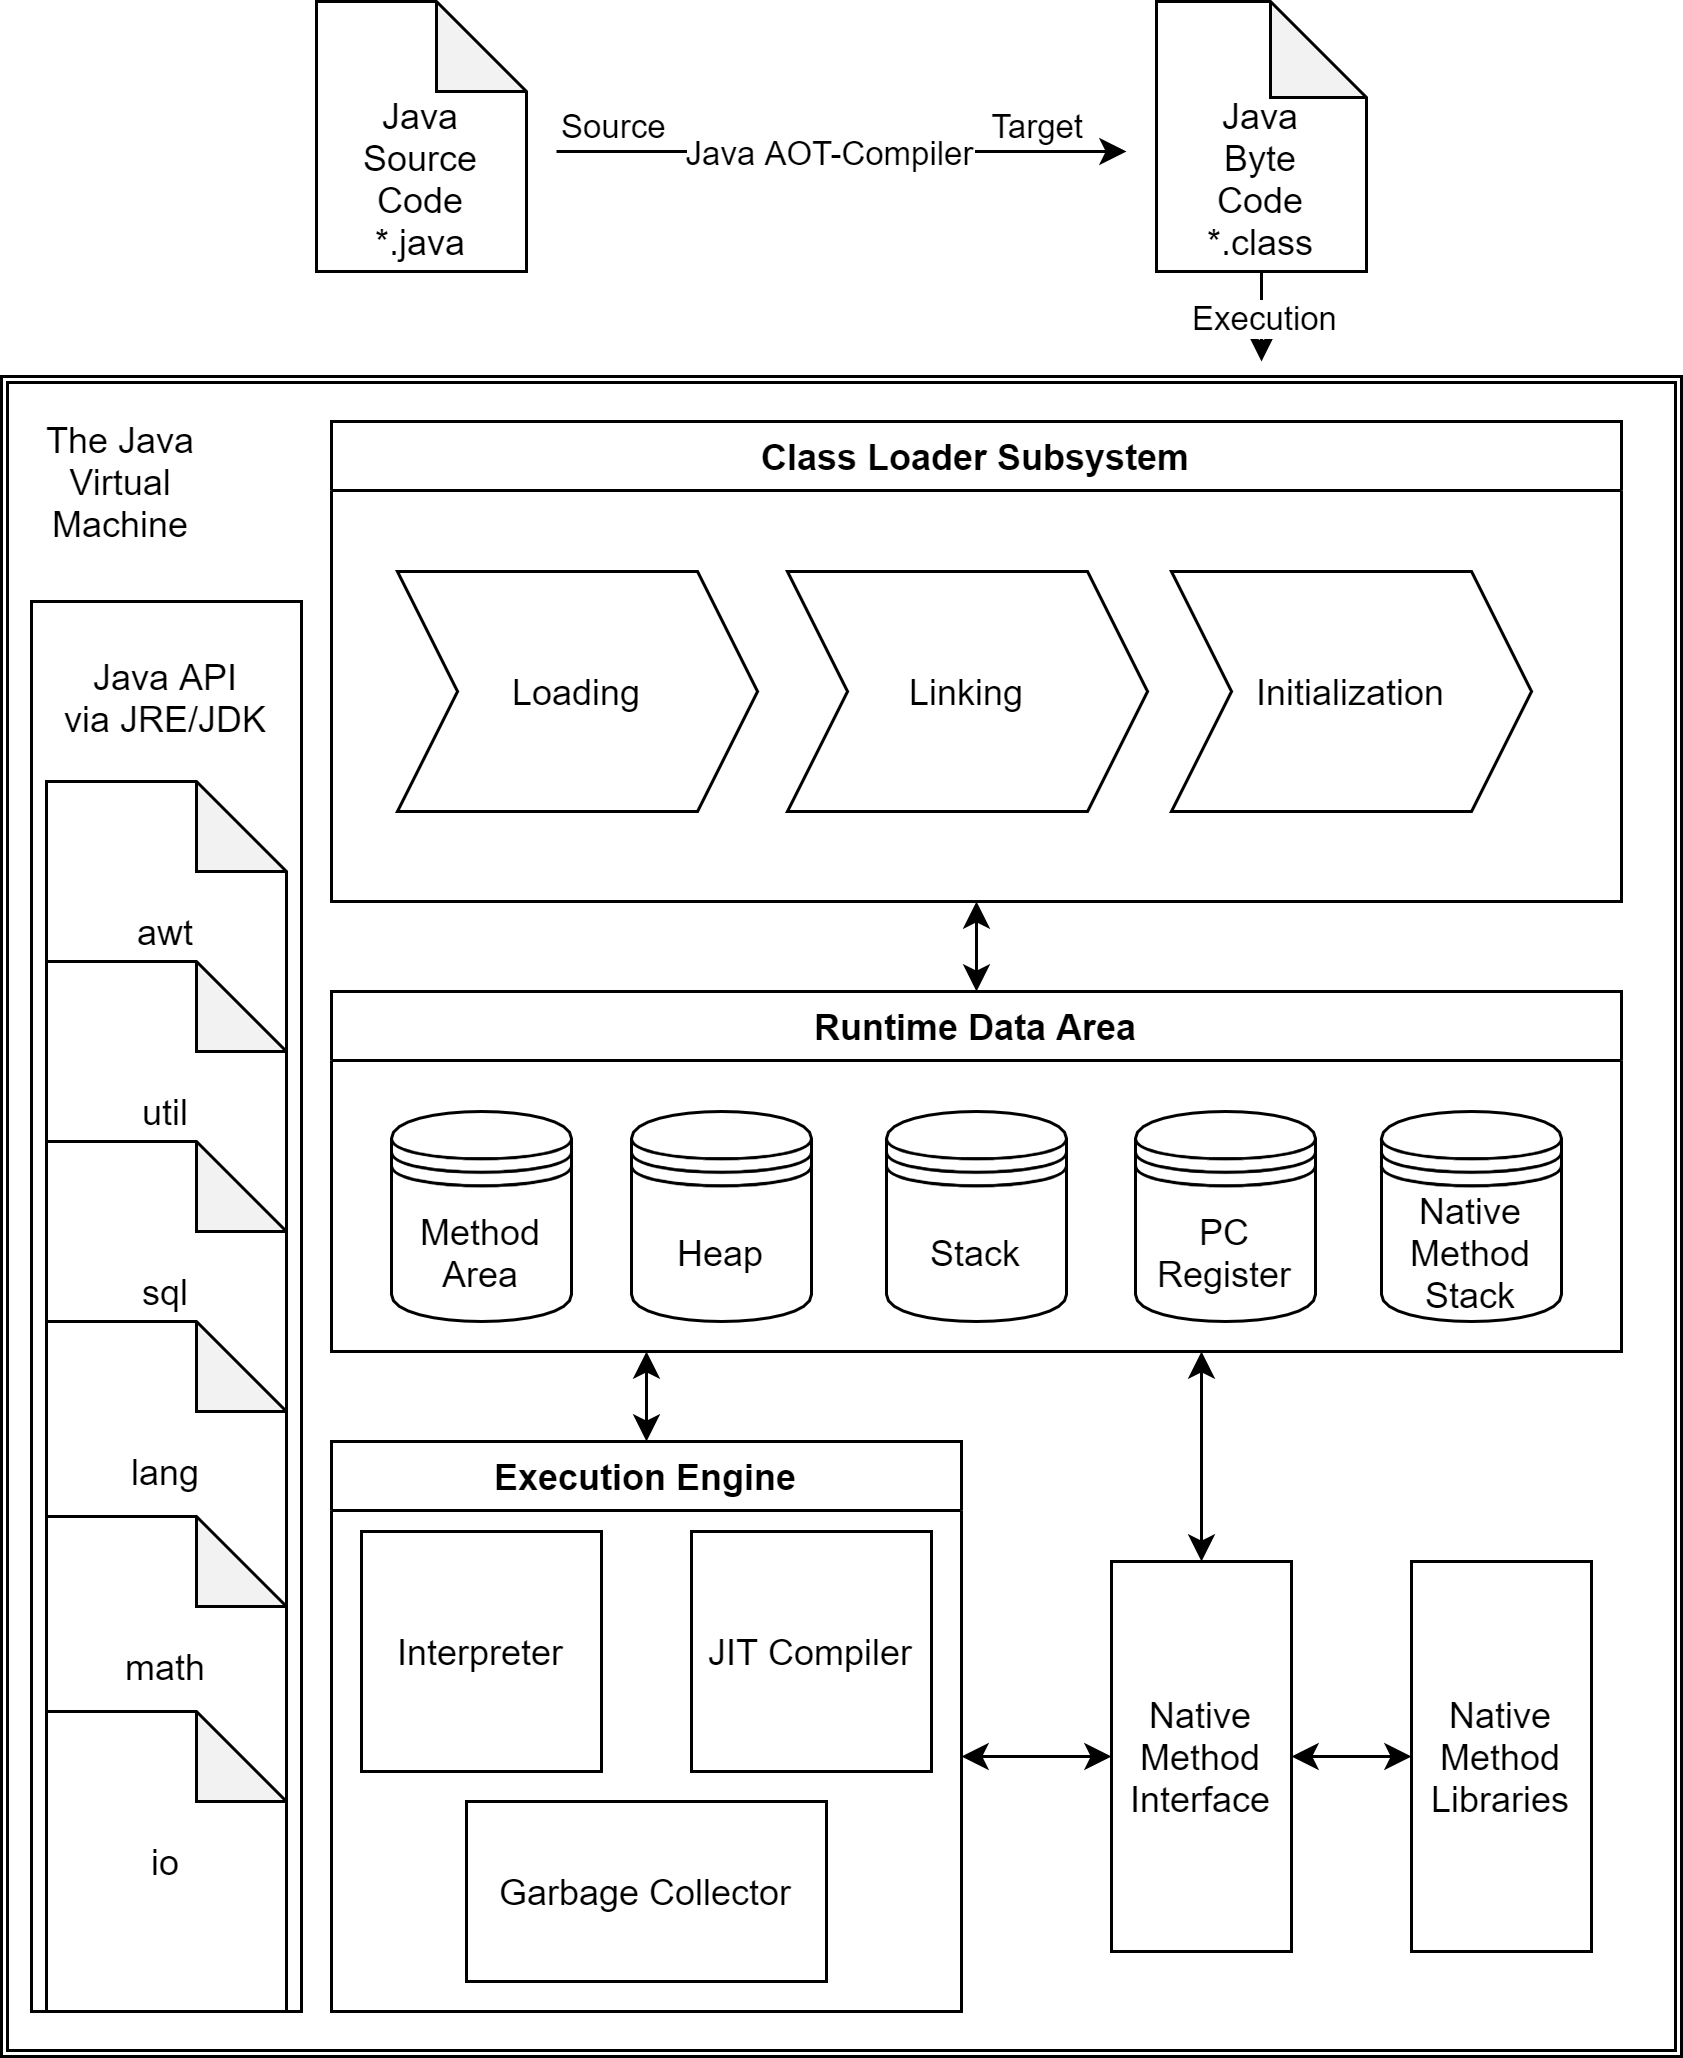
\includegraphics[scale=0.2]{../figures/JVM.png}
	\caption{The Java Virtual Machine simplified structure}
	\label{fig:jvm}
\end{figure}
When talking about the JVM the mentioning of classes and interfaces is inevitable.
In further parts the distinction between class and interface is abbreviated as class.
Multiple causes for class creation exist. The class to be created can be referenced by the constant pool of another class or a class' method can be invoked via reflection.\\
The creation at the start of a program works via loading the initial class and initializing it and furthermore invoking the specified method \emph{static void main(args[])}. The complete execution is driven by this method which, as soon as the program has more than this specific method and starting class, causes loading, linking and initialization of additional classes and invoking additional methods. How do the three steps, loading, linking and initialization work? The next paragraph talks about the beginning of a class creation and loading.\\
When creating a class in execution the JVM transforms the implementation-independent bytecode into an implementation-specific internal representation of the class. The algorithm is executed step by step meaning that a class has to be completely loaded before linking can be started and it has to be verified and prepared to the full extant before initialization.\\
The loading is started by the class loader which can be the JVM bootstrap loader or a user-defined one. Before the JVM starts the class loader it checks whether the pair binary class name and class loader already exist in which case the class already exists thus eliminating the necessity of class creation. If creation proves necessary the class loader has to find the class' bytecode representation on the specific platform, usually a file with the class' name in a hierarchical filesystem. After finding, if not a specific error is thrown, the JVM parses the bytecode, which in turn might not be valid resulting in different kinds of errors. Optional superclasses may also be resolved. After these steps the pair of loader and class are saved by the JVM. Loading usually concerns the class itself however linking concerns the whole ecosystem of the respective class. \\
The JVM links a class by preparing the class, superclasses, element type in case of array classes and resolving all symbolic references which as it is a recursive algorithm includes loading and linking these as well. The two strategies for resolution are an eager algorithm, meaning immediate loading and linking on verification, or loading and linking in a lazy way meaning resources are only loaded and linked when they are about to be used. At this point the JVM knows where the binary representation of a class can be found and which other classes are in the direct ecosystem of the class but the class' structure hasn't been checked yet.\\
Checking the class' structure is the main concern of the verification phase. In this step the class is checked for a static and structural constraints list. These include checks for appropriate type usage, number of arguments, instance initialization before usage, return types and many more. Any caught error in this step lead to ta thrown VerifyError. If no such error occurs the verification is finished and acknowledges the structual correctness of the binary class representation.\\
When doing the preparation of a class the JVM checks loading constraints on methods overriding those of superclasses and create and initialize static fields to default values. This phase can occur any time between creation and initializiation but imperatively before initialization.\\
Beforehand the resolution step with two different strategies has been discussed briefly without going into detail. This omission will be rectified now. Resolution in the context of the JVM means the process of dynamically determining conrete values from symbolic references in the run-time constant pool. The target of resolution includes classes, fields, methods, method types, method handles or dynamically computed constants. These different targets require different approaches. These usually require class loading, lookup, etc. They can also fail and throw errors or succeed resulting in a resolved dynamic binding in the constant pool. With all these preceding steps the class is now ready for initialization.\\
Conceptually initializing a class is fairly simple as it is the mere execution of the initialization method. This can only be invoked by certain cases or instructions like \emph{new} or a subclass is initialized resulting in the initialization of the superclass. At this point the JVMs multithreading needs to be taken in account since synchronization is imperative. This again is solely handled by the JVM and of no concern of the application programmer. The concrete inner workings are generally spoken handled by object states and unique initialization locks. The Initialization phase is the final stage of the class loader subsystem. Now the different data areas are explained briefly.\\
The JVM run-time data area is subdivided into five different data areas. These fulfill different tasks and are also different in their relation towards processes and threads as there are data areas being defined per thread and others per process. This results in some data areas existing as long as the JVM is running and some areas' existence is linked to their respective thread's existence. The data areas are, as can be seen in figure \ref{fig:jvm}, the method area, heap, stack, program counter register and the native method stack. The next paragraphs explain which area is responsible for which task and when they are created and destroyed.\\
The method area is shared between all JVM threads and is created on JVM start-up. It stores all per-class structures like the constant pool or field and method data.\\
The heap is a JVM-defined structure, as such is created on JVM start-up, and is shared between all threads. It is an allocation space for class instances and arrays on run-time. Allocation and deallocation in the JVM is automatically handled by the garbage collector which again can be shortly defined as an automatic storage management system. The structure of the heap is not necessarily contiguous and attributes like initial, maximum and minimum size can be defined by the programmer or user.\\
The stack is a thread-defined structure and is itself subdivided into thread-specific stacks. It does have a fixed size which is defined at stack creation. Regarding the data a stack holds: local variables, partial results and has its share in method invocation and return. The not necessarily contiguous stack is only changed by pushing and popping frames.\\
The program counter (PC) register holds the current program counters of all running threads. A thread specific PC register contains the address of the thread-specific currently executed method.
The native method stack is an optional data area not supported by all JVMs. If they are supported they are conventional stacks on a thread basis. They can be of fixed or dynamic size. These stacks fulfill a similar task to the regular stacks but are for code not written in Java.\\
With the data areas explained the execution engine is the focus of the next few paragraphs.\\
The execution engine is mainly built up of three different components, the interpreter, the just-in-time (JIT) compiler and the garbage collector.\\
The interpreter is the part that executes the code directly/live including byte code getting translated to actual implementation-dependent machine code and its execution on the central processing unit (CPU) per instruction. This mechanism causes the interpreter to reinterpret, translate and execute the same code multiple times per instruction, code which is redundant work making the interpreter slow in comparison to AOT-compiled execution. When doing so the interpreter of the JVM profiles the run code for example by keeping track of how often a certain piece of code is executed. This profiling information is then used to choose the parts of code that get JIT-compiled hindering too many redundant interpretation steps.\\
A part of the byte code chosen for JIT-compilation is compiled to machine code and gets thus turned from implementation independent form into implementation dependent form. Afterwards if this part of the program gets executed again the machine code gets executed directly out from the cache where it's stored in the meantime. This method of choosing code hotspots that get executed often for compilation rather than continuous interpretation is called adaptive compilation and is used in the Oracle Hotspot VM.\\
The last component left out so far is the garbage collector (GC). It takes care of objects without references resulting them to be unreachable by application code. Such an object will be removed by GC and memory will be freed up. The GC is part of inner workings and fully functions without user interaction but the programmer can make a not guaranteed call for the GC.\cite{Lindholm}\\
This section explained the JVM ecosystem. It is split up between an AOT-compiler that creates Java bytecode out of Java source code. From there on the JVM executes the bytecode. Generally speaking the JVM consists of three areas, the class loader subsystem, taking care of loading, linking and initialization, the runtime data area and the execution engine, consisting of the interpreter, the JIT compiler and garbage collector. Aditionally to ease the programmer's work the JRE or JDK come with an API. What hasn't been discussed so far are technologies for making Java execute faster. These technologies are a core feature of GraalVM which is the topic of the next section.
\section{GraalVM}
\begin{figure}
	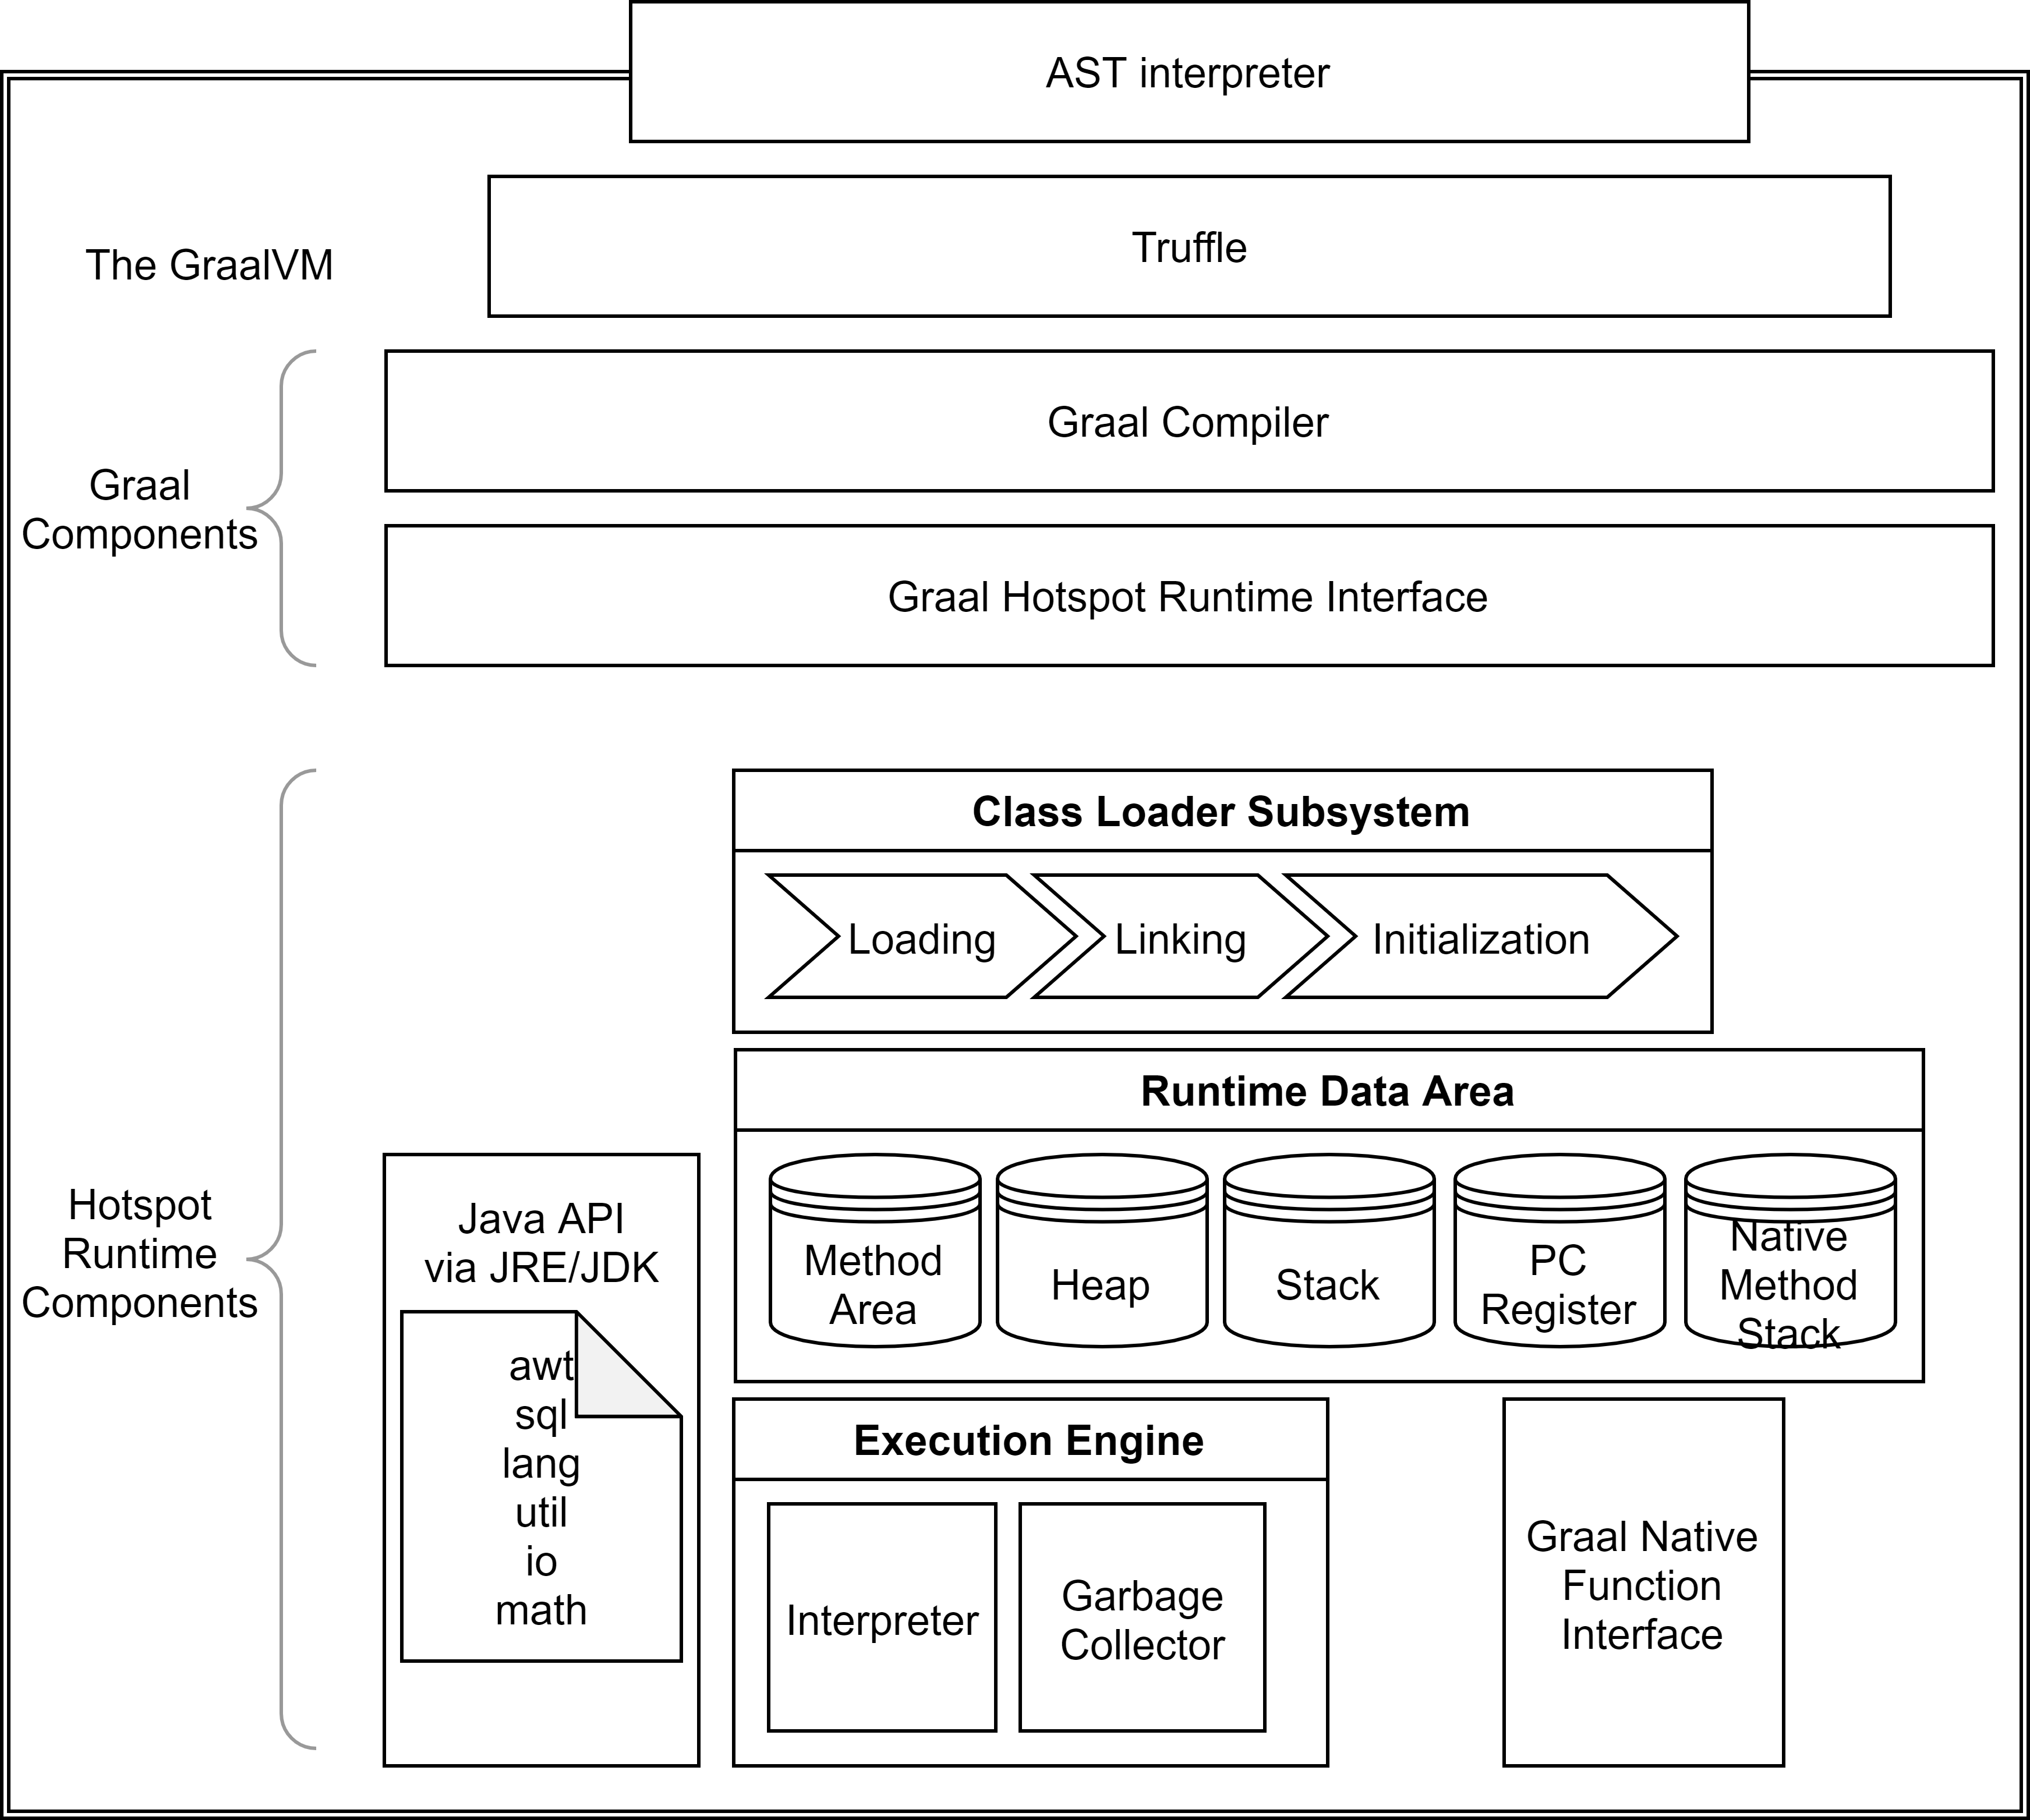
\includegraphics[scale=0.2]{../figures/GraalVM.png}
	\caption{The Graal Virtual Machine simplified structure}
	\label{fig:graalvm}
\end{figure}
As seen in the last two sections building a virtual machine for executing programming languages is a non-trivial task needing a lot of effort. A lot of this effort has to be redone for different programming languages. The core idea of GraalVM is to reduce this effort via a layered structure where each language implementation is in essence an abstract syntax tree (AST) interpreter via the Truffle API. All low level implementions like JIT compiling, data areas, memory management, optimizations and the like are reused by each language implementation connecting to the GraalVM or any JVM via Truffle. Considering performance these implementations are best run on top of GraalVM. Reasons for that are explained in the next section.\\
The GraalVM complete ecosystem is comprised of multiple technologies. In the runtime environment the GraalVM reuses most components from the HotSpot VM like the class loader subsystem, the runtime data area and parts of the execution engine, in particular the interpreter and the garbage collector, but replaces the HotSpot JIT compiler with the GraalVM compiler. Since the GraalVM compiler functions differently it also implements an interface between the regular HotSpot components and the GraalVM compiler. Outside of the VM it also has the Truffle framework for different language implementations. Already implemented languages are JavaScript, Ruby, R, python and LLVM-based languages like C, C++ and Rust. Thus the feature is able to end the segregation of programming languages. Another feature is its ability to be embedded in combination with OpenJDK, node.js or inside Oracle Database, while also being able to be run standalone.
\subsection{GraalVM Compiler}\label{sec:graalcomp}
The GraalVM Compiler replaces the JIT compiler in a JRE. Other as the regular java JIT compiler it doesn't translate java bytecode directly to machine code but to the Graal IR. \cite{inproceedings} The Graal IR is a graph-based high-level intermediate representation. This intermediate representation is key to GraalVM's aggressive optimization techniques based on optimistic assumptions such as specific types and branch prediction. Aggressive optimization also means the compilation is prone to failures which are caught by so called guards. When a guard fails execution is transferred back to interpretation. This mechanism is called deoptimization. \cite{ChambDeopt} Compiled code gets saved as a VMs internal data structure and subsequent calls to the particular part of code get always directly executed in machine code omitting the unnecessary step of interpreting.\\
Another component the GraalVM project substitutes is the Java Native Interface \cite{Lindholm}. It is exchanged with the Graal Native Function Interface (GNFI). \cite{grimmerNative} It allows for efficient native function calls within Java code.
\subsection{Truffle API}
The Truffle language implementation framework enables programmers to write an AST interpreter in Java for any programming language. The biggest advantage is the reuse of JVM runtime services such as automatic memory management with execution by a JVM. But how does the interpreter work?\\
The interpreter works by modelling language structures as nodes building the abstract syntax tree. Evaluation of the tree works by invoking the execute method which is within every type of Node. These different Node types all extend the class Node forcing them to have an execute method implementing their respective semantics. The whole tree gets then recursively evaluated by the recursive execute method calls.\\
Optimizations on AST level mostly work with a speculative specialization technique. The Nodes rewrite themselves into specialized variants at run time where profiling information is available. \cite{wuerthSelf} As we have discussed earlier in the GraalVM compiler speculative optimizations, like a specialization, are prone to failure. Instead of going just back to interpretation a failed specialized Node rewrites itself back into a more generic version. What kind of specializations are possible via this approach?\\
Type specialization especially with dynamic languages is an operation reducing code on runtime and thus creating speed up. To discuss this optimization method further the add method with the + operator in the scripting language JavaScript is used. The add method in JavaScript is defined for various types including Strings and Numbers. We reduce the language's complexity to the forementioned two types in the example.\\
\begin{lstlisting}[caption=JavaScript addition types minimal example]
	var w = 1 + "Test" // results in "1Test"
	typeof(w) // string
	var x = 1 + 2 + "Test" // results in "3Test"
	typeof(x) // string
	var y = +"1" + 2 // results in 3
	typeof(y) // number
	var z = +"Test" + 1 // results in NaN
	typeof(z) // number
\end{lstlisting}
The above example code shows how addition in JavaScript works. The interpreter has to check the types of two operands from left to right before it can decide on which operation to use, an addition for numbers or one for strings.\\
\begin{figure}
	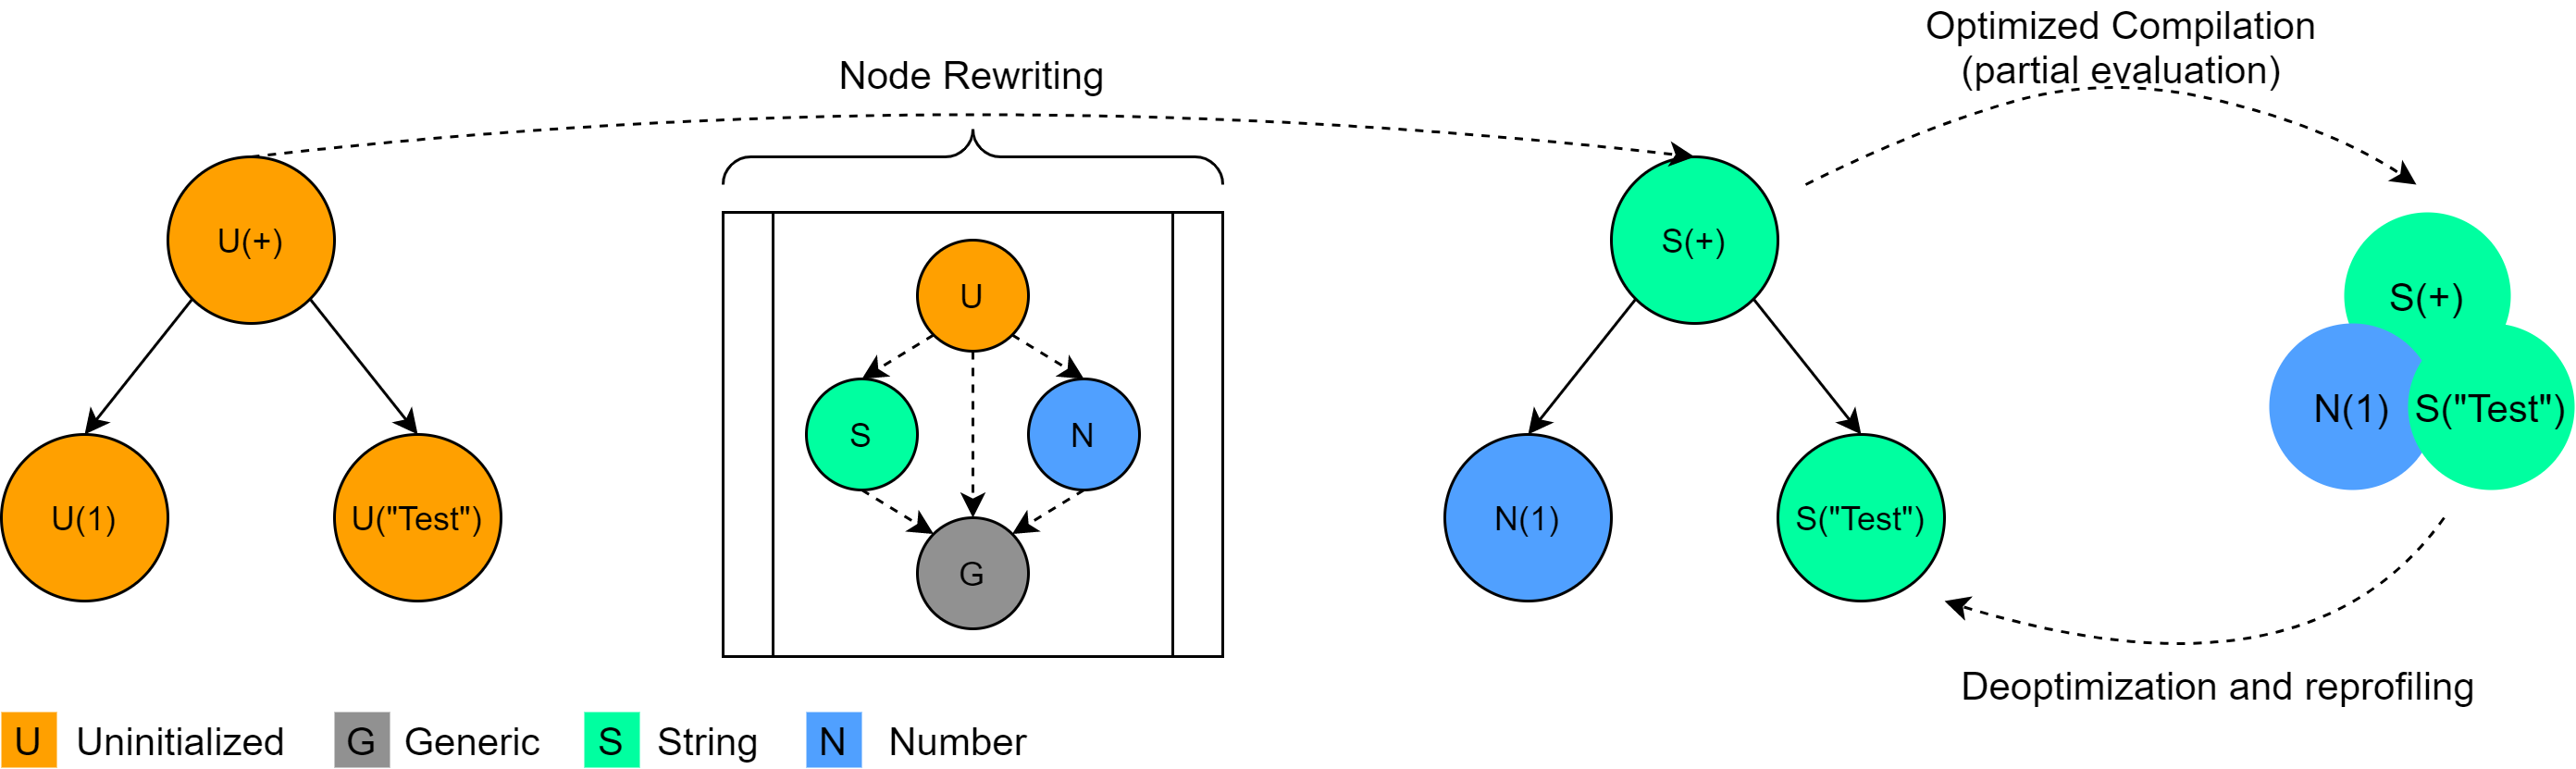
\includegraphics[scale=0.165]{../figures/NodeJIT.png}
	\caption{Simplified Node Rewriting example \cite{VMRule}}
	\label{fig:trufNR}
\end{figure}
The node rewriting process shown in figure \ref{fig:trufNR} happens at various state to achieve different goals. In the interpreter node rewriting is used to capture profiling feedback via runtime information such as the rate of node rewrites. If certain thresholds are surpassed the specialized AST gets compiled into machine code. If the execution fails the compiled code gets deoptimized back to the AST interpreter where again nodes are rewritten and now update the existing profile information. After this step the newly specialized AST gets compiled again.\\
One note on the compilation process: The compiler uses as said aggressive optimization methods. This operation is successful for stable ASTs. Then compilation techniques like method inlining and eliminating interpreter dispatch code can be performed. This technique is called partial evaluation.\\
In addition to type specialization truffle offers so called polymorphic inline caches. \cite{ChambOpti} An inline cache itself is simply caching a method from a former lookup at call site. In Truffle inline caches are built by chaining nodes which check for cached target matches which are then executed. At a predefined chain length the chain gets replaced by a polymorphic node handling all operations.\\
As discussed in the JVM section program loading often requires resolution. An implemented truffle language can cache resolved targets at run time by replacing an unresolved node with its resolved version. Thus further resolutions of this node are prevented which leads to an optimized version of the AST.\\
This section gave a small introduction into the Truffle API for implementing languages via an AST interpreter for running on top of a JVM and showed the optimizations that are conducted on AST level. After an AST at run time becomes stable with no more rewrites the AST is compiled dynamically to machine code. Truffle uses the JIT compiler of a JVM, in case of GraalVM the GraalVM compiler. If GraalVM is used the nodes' execute methods are inlined producing one compilation unit of the whole tree. In the next step the GraalVM compiler uses its aggressive optimization techniques for the whole inlined tree unit producing efficient machine code. These combined methods are based on the principle of the first Futamura Projection also called partial evaluation. \cite{FutaPart} As stated in section \ref{sec:graalcomp} guards or also optimization points need to be implemented to check all the assumptions made before compilation. As soon as it is necessary to rewrite a node during machine code execution the control flow gets transferred back to the interpreted AST to rewrite the node either on profiling information to another specialized version or a more generic version. \cite{ChambDeopt}

In conclusion the GraalVM project aims at simplifying language implementations and application programming while also trying to have a performant run time. The simplification comes from introducing a framework for implementing languages as AST interpreters which can run on top of any JVM. The performance comes especially from running the AST interpreter on top of the GraalVM which uses various techniques to bring run time performance to higher levels.
%\begin{tikzpicture}[nodes={draw, circle}, ->, minimum size=2cm, level distance = 2.5cm, sibling distance = 2.5cm]
%	\node[fill=lightorange] (p) {U(+)}
%		child { node[fill=lightorange] (n) {U(1)}}
%		child { node[fill=lightorange] (s) {U("Test")}};
%\end{tikzpicture}
%\begin{tikzpicture}[nodes={draw, circle}, ->, minimum size=2cm, level distance = 2.5cm, sibling distance = 2.5cm]
%\node[fill=lightgreen] (sp) {S(+)}
%child {node[fill=lightblue] (sn) {N(1)}}
%child {node[fill=lightgreen] (ss) {S("Test")}};
%\end{tikzpicture}\\ \\
%\begin{tikzpicture}[sibling distance=1cm]
%\node[fill=lightorange, label=right:{Uninitialized}] (u) {U};
%\node[below=.3cm of u,fill=lightblue, label=right:{Number}] (n) {N};
%\end{tikzpicture}
\section{Graal.js}
The Graal.js project is an AST interpreter on top of Truffle. It is in full compliance of the newest ECMAScript 2020 language specification \cite{kangax1, GraaljsComp} and growing support of the technical committee 39 (TC39) proposals for future ECMAScript language specifications. \cite{kangax2, gitTC}  The runtime can execute JavaScript and Node.js applications with the previous discussed benefits of the GraalVM technology stack. \cite{Graaljs} As a recap the most notable ones are performance and polyglot programming support with multithreading support.

\section{ECMAScript modules - Current state}
With ECMAScript 6 the language got modules making it possible to divide code up into multiple files. Although this possibility has been around in JavaScript before, it was implemented by external libraries and not an inherent specified feature. The ability to import modules as needed came with a rise in source code size in regular JavaScript programs. When the language started out it was not unusual to have a one-line .js (JavaScript) file. As the code size rose the necessity of modules came with it which led to a multitude of concurring solutions. As script concatenation as the basic step meant manual building and testing the method could only be used in simple projects while more difficult ones started using module loaders. Those in turn could also become complicated for larger code bases. To overcome these problems so called module bundlers, like Babel, could be used to generate the needed JavaScript code at build time. Thus the code includes all dependencies in a single concatenated file. The specification of modules in ECMAScript bundled these efforts into one concept and gave implicit module support by the language. With this specification performance of module loading was pushed towards engine implementation.

In a short note to avert term mixup. ECMAScript is a language specification for script languages. The actual code written is in JavaScript and this language is then run via engines in browsers on computers. So in hard terms an ECMAScript specification does not need to be fully supported by a particular browser and single features sometimes are left out but in general engine implementation follows the ECMAScript specification leading to the specification's features in JavaScript sourcecode.

In a broad sense modules at current state read like regular scripts with the difference of them being in strict-mode only and possible usage of imports and exports. The benefits are separate files with self-contained functionality, sharing of those files between different projects, diminishing naming conflicts, obvious naming conflicts and the robustness that comes with shared open source. But what are modules in the context of JavaScript in detail?

As a module is run in strict mode all declared variables, functions and classes are private and cannot be accessed from the outside. Only those top-level items that are explicitly exported by the keyword \emph{export} can be used from a script importing the module. This is then done by the keyword \emph{import} either the whole module or explicitly named items which can also be aliased.

As modules have to be loaded and are sometimes scattered throughout the web, deferring module loading is a default setting. Another note is the caching of modules. A module is only executed the first time it gets imported. All other scripts importing the module are given the already evaluated exports. This also means that a change in one of the exports is visible to all importing scripts.

This standard unfortunately left out the possibility to add inline modules into a script which results in modules just containing one exported function. This results into unnecessary files which could be avoided by inlining the module into the original script. This exact feature is discussed in the next section.

\section{Proposal: Module blocks}
Module blocks are a TC39 stage 2 proposal from Daniel Ehrenberg and Surma. \cite{gitMB} As stated ECMAScript does not have the feature of inlining modules. This cause several issues in programming applications, most notably code composition and file count. In the current state if code should be run in parallel an additional file is needed resulting in every Worker needing a separate file. So module blocks work like a module but are inside the script where they are also imported. One important note to take is the non closure of module blocks following the principle of coding in one place, running it anywhere. It can thus also be imported from any Realm and is code independent of a particular context. So in a sense module blocks are mainly a syntactical addition to ECMAScript as the concept is to provide a syntax for inlined module contents. These can then afterwards be imported asynchronously. Reason being the ability of module blocks to import other modules as well. As regular modules since ES6 module blocks will be cached in the module map after the first import. One note to take is, that module blocks need to be imported via dynamic import() calls rather than import statements. This is due to them not being addressable as specifier strings.\\
\begin{figure}
	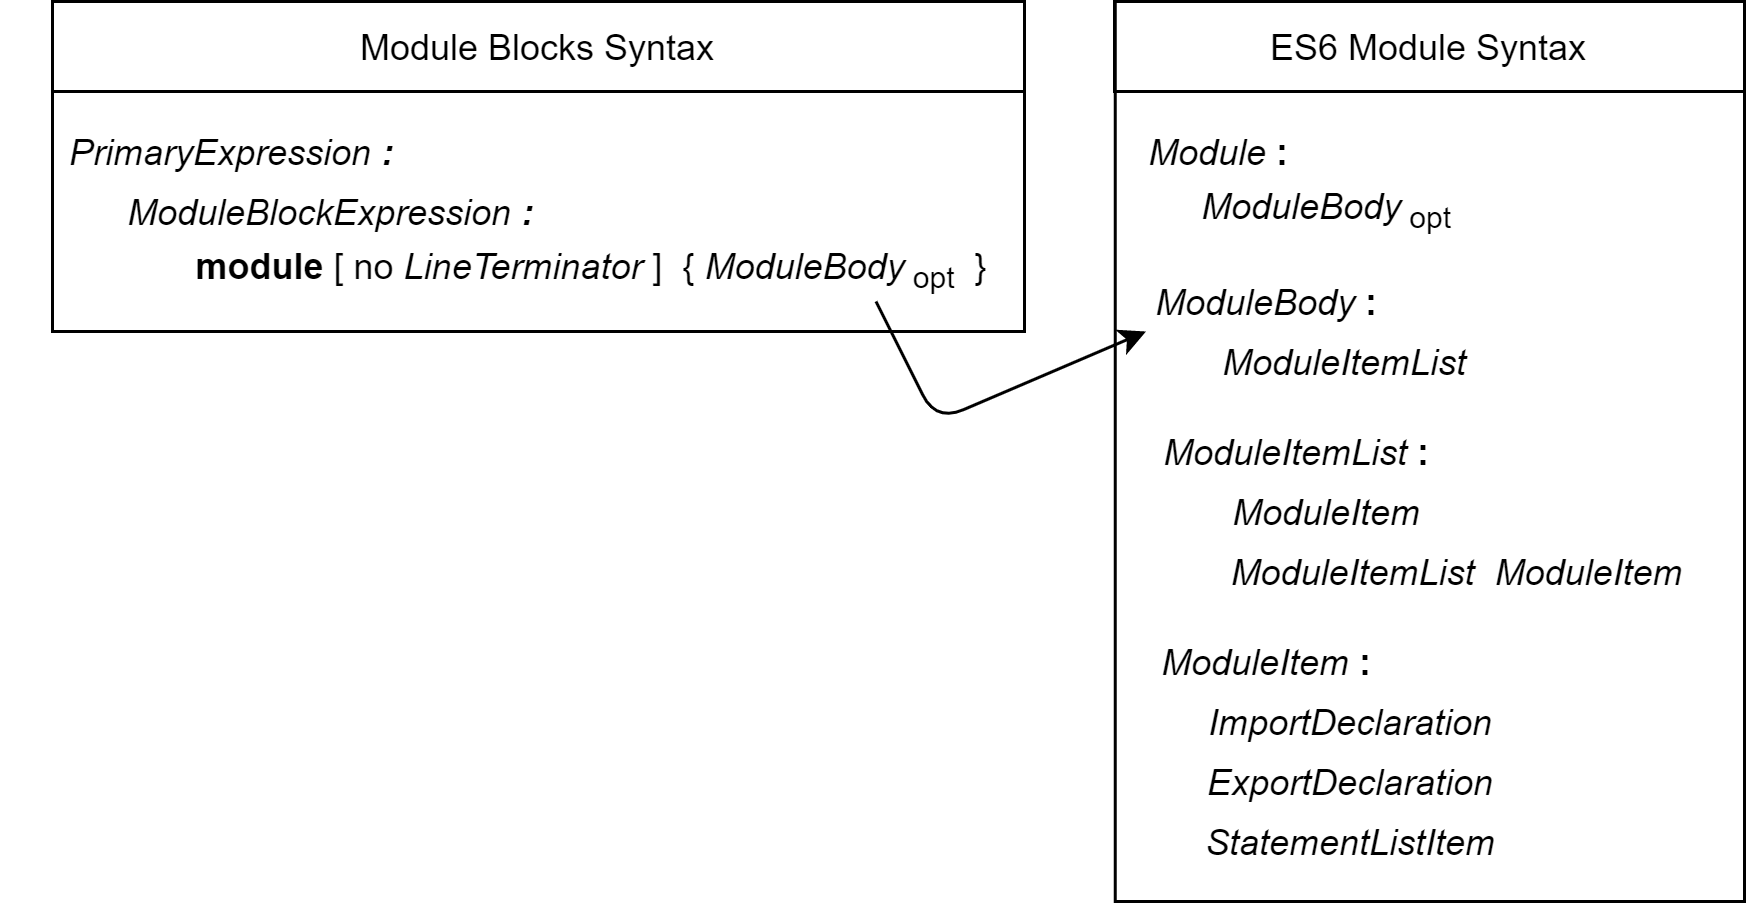
\includegraphics[scale=0.165]{../figures/ModuleSyntax.png}
	\caption{Syntax of Module Blocks and ES6 Modules \cite{gitMB, ecma}}
	\label{fig:mbSyn}
\end{figure}

\chapter{Implementation}

This chapter lays out the implementation by presenting an architectural overview on how and where the proposal can be included in the Graal.js project. This inclusion is further detailed in the upcoming sections. The implementation explanation is then wrapped up by explaining the interaction with dynamic imports and the serialization / deserialization framework.

\section{General overview}
Before thinking about implementing the proposal in the Graal.js project one needs to know how source code is evaluated by Graal.js. The path of source code going through the engine is straightforward. Without going too deep into the specifics it follows Figure \ref{fig:mainImpl}. The source code is traversed and transformed into a token stream. This token stream is then evaluated by the parser which uses the identified tokens in conjunction with the specified grammar given by ECMAScript \cite{ecma} to transform them into an intermediate tree form. This tree contains nodes representing general language concepts without specifying the nodes into specialized forms. As can be seen in Figure \ref{fig:mainImpl} a module block is represented by a function node in the intermediate form. Later on in the translation pipeline the \texttt{GraalJSTranslator} class is called with an intermediate form node and translates it into a specified module block node. In the scope of this thesis a \texttt{FunctionNode} to a \texttt{ModuleBlockNode}. These specialized nodes are then executed when being visited in the tree. On the specifics of interpretation and compilation during execution see Section \ref{sec:graalcomp}. 

\begin{figure}[h!]
    \centering
    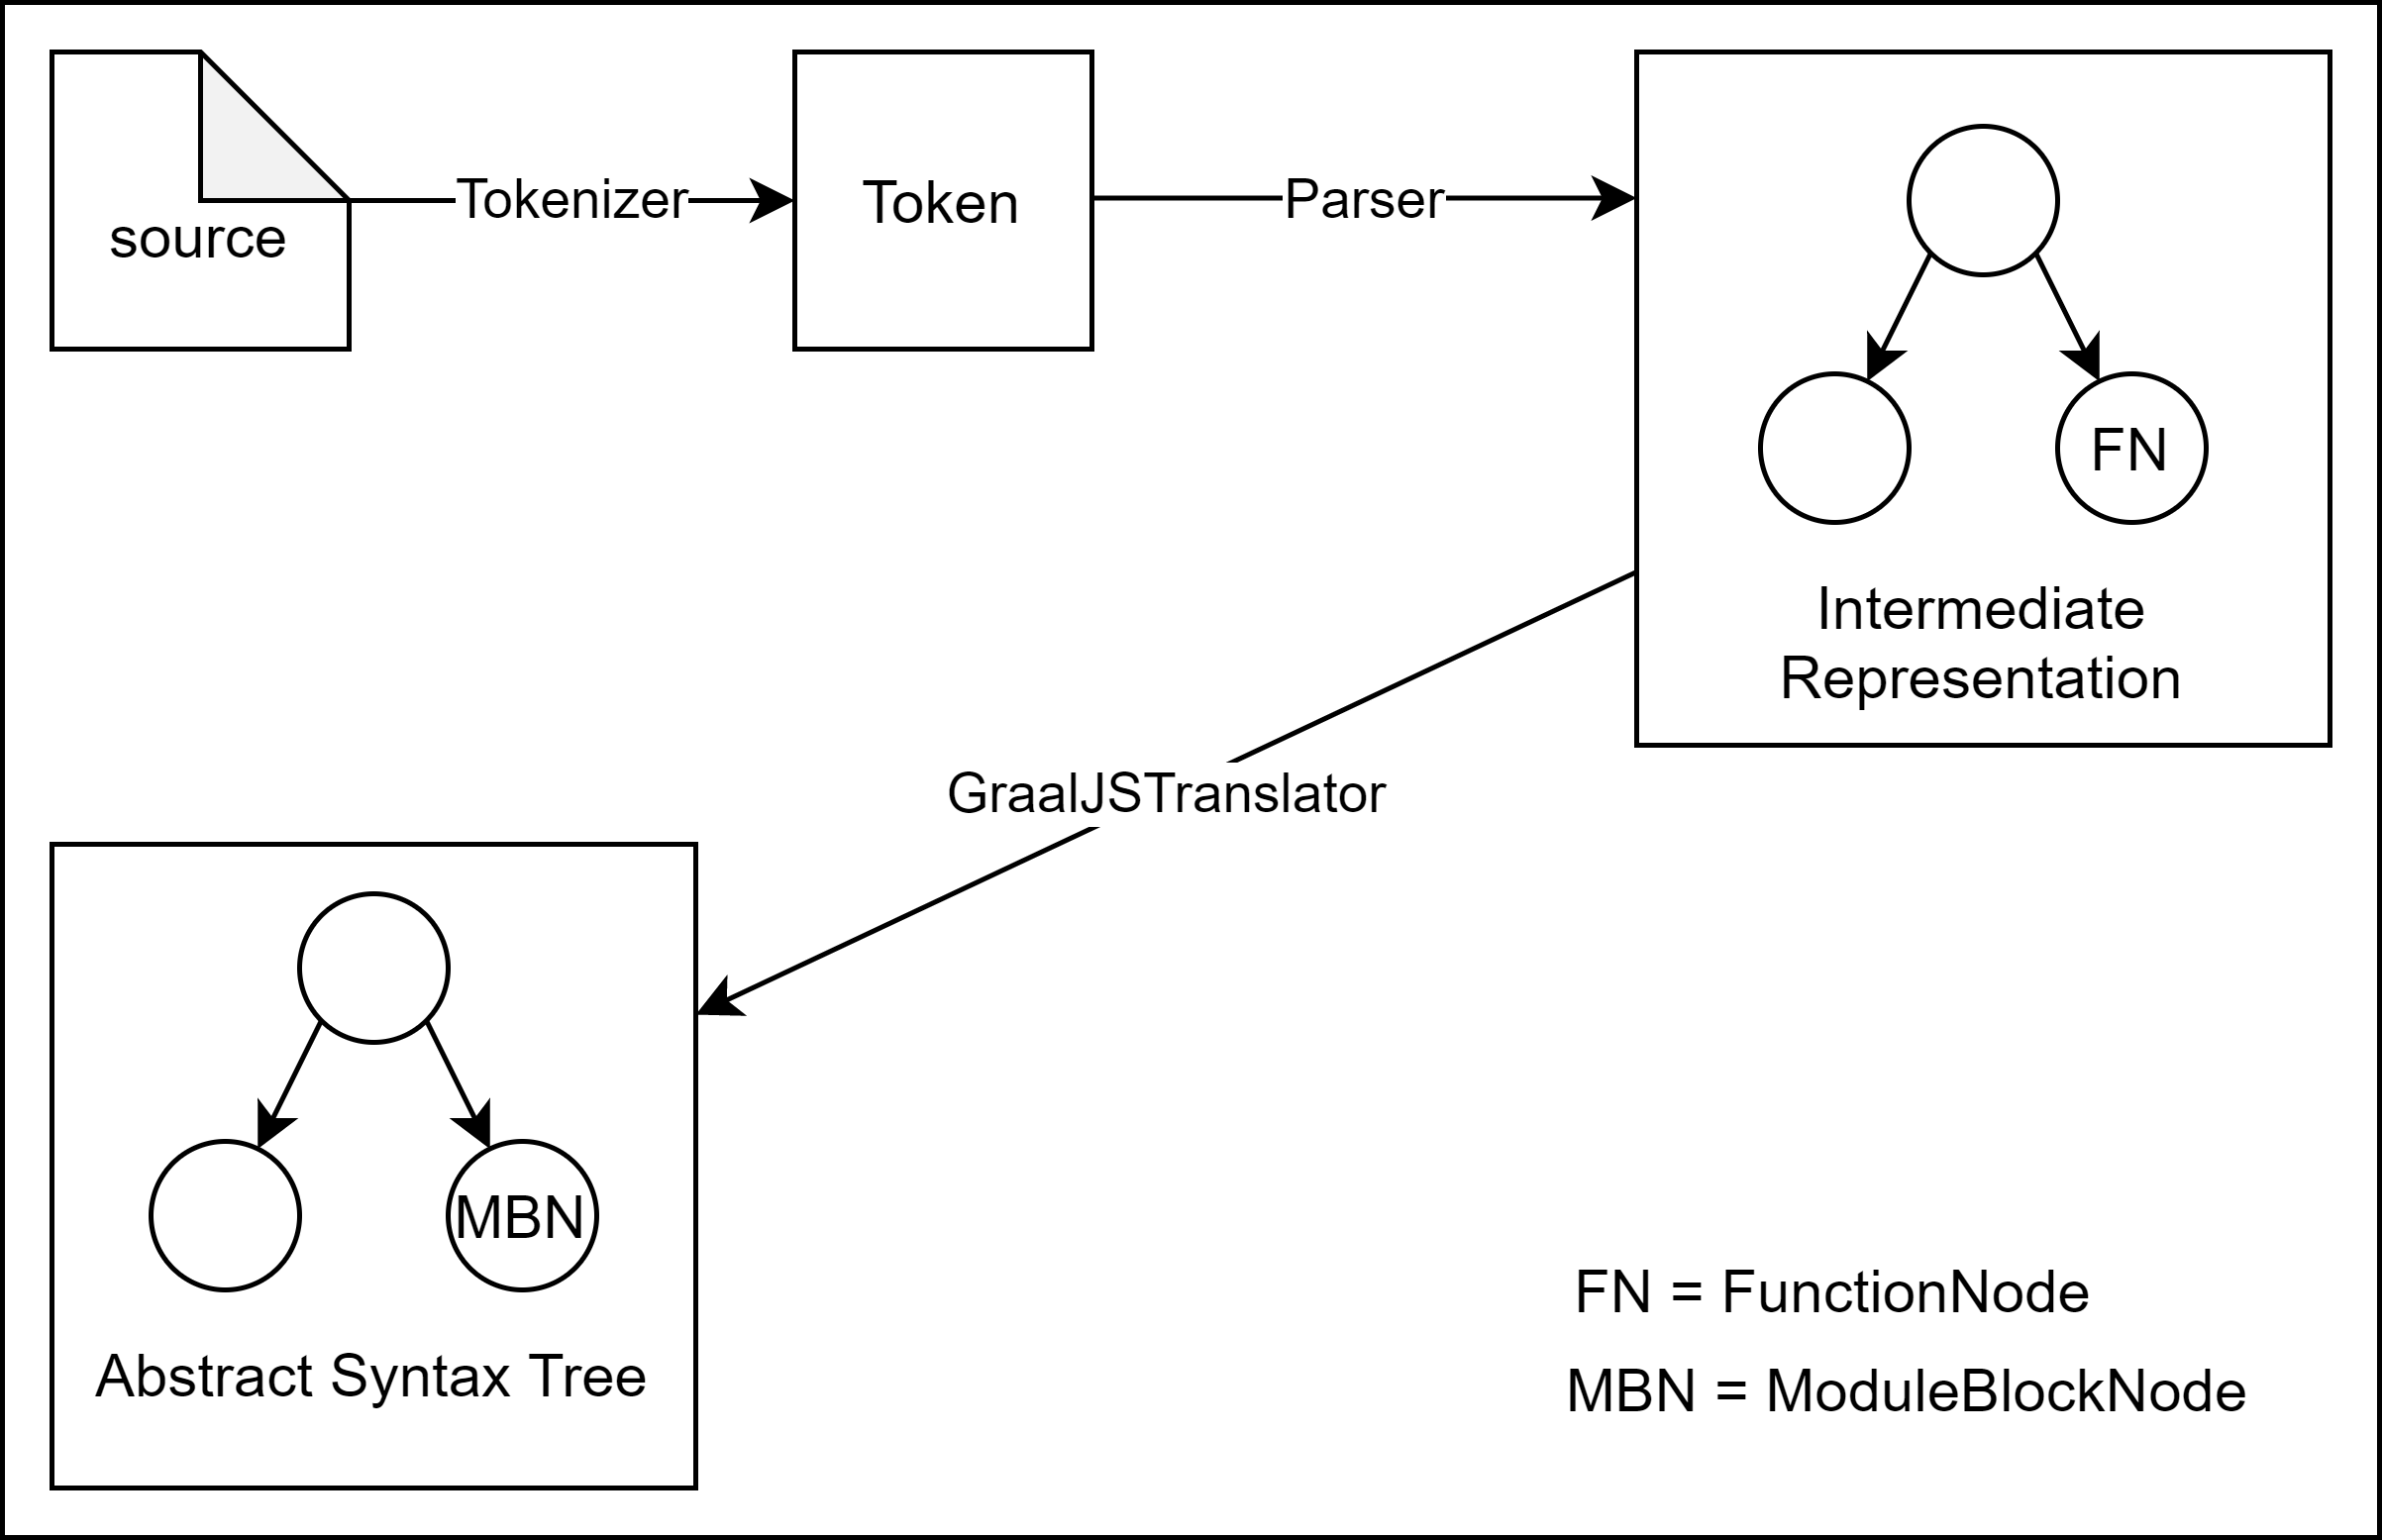
\includegraphics[scale=0.165]{figures/implMain.png}
    \caption{Code evaluation by Graal.js}
    \label{fig:mainImpl}
\end{figure}

Implementing the module block proposal into the Graal.js project involves several steps. Those are adjustments to the parser to capture the newly introduced syntax, implementation of the prototype, introducing a new respective node for module blocks and lastly adjusting the node for dynamic import-calls. At this point the implementation is limited to the available specification of the proposal. The chapter's outline is firstly the module block direct implementation into the Graal.js project followed by explanations of some necessary adjustments for dynamic import-calls. The direct implementation part is split up in four parts: parser changes, module block node, constructor and the prototype.The specific parser changes are explained in the next section.

\section{Parser}
From the specification we can take away that \texttt{module} won't be introduced as a keyword in ECMAScript meaning during parsing the token "module" will be treated as an identifier. As both identifier and module blocks are classified as so called \texttt{PrimaryExpressions} the main change is happening in this explicit parser method inplace of the "ident"-Token branch. Like Listing \ref{lst:impl:minModule} shows \texttt{module} can still be used as identifier. Thus recognizing a module block needs a lookahead token and additionally satisfy the no line delimiter condition. This is done by first checking for the next token being a \texttt{\{} after a \texttt{module} identifier , changing from the "ident"-branch to the module block branch and then checking whether there is at least one line delimiter between the \texttt{module} and the \texttt{\{}. A line delimiter occurrence would result in a syntax error. Otherwise the parsing continues with capturing all statements inside the module block similar to a regular module and then putting the result into the same intermediate representation form a regular module would be put in. This caters to the notion of modules and module blocks acting similar in the language specification. The only relevant difference is the end of the parsing which is the end of file in the module case and a closing brace (\texttt{\}}) in the module block case. The next section talks about further steps that are taken during translation.

\begin{lstlisting}[caption={Minimal module identifier example in JavaScript}, label={lst:impl:minModule}]
    var module = 42;
    
    var moduleBlock = module { };
\end{lstlisting}

\section{ModuleBlockNode: Module Blocks' Truffle AST representative}

The Graal.js project includes a class called \texttt{GraalJsTranslator}. This class is responsible for translating the intermediate representation nodes into specialized ones for the resulting AST. During execution of this class the intermediate module block representative gets translated into a module block node. The node is built according to the provisional proposal's specification meaning the hidden properties are set as defined. At the current point the \texttt{hostInitializeModuleBlock}-method which is mentioned in the specification is not implemented as it is not included in the specification yet. With the node representation itself finished the next section turns towards the prototype and the constructor.

\section{ModuleBlock prototype and constructor}

This part of the implementation is split up into two parts where firstly a discussion is depicted as to why the constructor is specified as is. Secondly the actual implementation is explained. At current state, as of July 2021, it is unwished for by the developers to implement yet another eval-esque structure coming from the desire for less dynamic evaluation. A point for including an actual constructor for module blocks would be the symmetry and consistency in the whole language's specification. This concern can be brought up since structures like \texttt{AsyncFunction} or \texttt{GeneratorFunction} do have constructors with a code-string parameter. Right now the eval-point outweighs the symmetry-/consistency-point. The constructor when called simply throws a type error. This concludes the rather simple implementation of the constructor with the discussion behind it maybe resulting in a change of the constructor's specification. The next paragraph concludes the implementation of the module block itself by introducing the module block prototype.

The prototype is constructed in a fairly simple way. Its prototype property is the module block Prototype Object with the general attributes writable, enumerable, and configurable all set to false as is standard in the ECMAScript specification. The module block Prototype Object is \\ \texttt{\%ModuleBlock.prototype\%}. Its internal prototype slot is \texttt{\%Object.prototype\%} and it is an ordinary Object. It has simply one function which is the toString() method. This method should check whether it is used on a \texttt{ModuleBlock} object and as such return the hidden \texttt{SourceText} property.
On a second note \texttt{ModuleBlock} is specified as global. This allows for the code in Listing \ref{fig:globModule} to work. Again this matter can be subject to change during the proposal's progress.

 \begin{lstlisting}[caption={ModuleBlock working as global in JavaScript}, label={fig:globModule}]
        var moduleBlock = module { };
        
        moduleBlock instanceof ModuleBlock; // true
\end{lstlisting}

This concludes the module block implementation itself. The module block's syntax is implemented in the parser, the module blocks runtime semantics are implemented in the specified module block node for the resulting AST and the constructor's and prototype's specification is met accordingly with also registering \texttt{ModuleBlock} as global. In conclusion the module block at this state is implemented as a standalone without much interaction with the rest of the EcmaScript ecosystem. This leads us to the question how does the module block interact with existing language features. The proposal's specification only states one interaction with another language feature: the import()-call. Thus the next paragraph states the necessary changes for integrating module blocks into the dynamic import calls.

\section{Interaction with dynamic import}

The interaction between module blocks and dynamic imports points to the Graal.js representative for dynamic imports, the class \texttt{ImportCallNode}. Hence, the class needs to be changed in this matter. The main difference is the change from using only Strings with the module's URL as identifiers to using the module block node as identifier for the resulting Module Record. To accomplish this, the object needs to be checked and if it does not satisfy the condition of being an object with the internal slot of \texttt{ModuleBlockBody}, a String is then used as identifier, otherwise the \texttt{ModuleBlockNode}. After that the regular \texttt{HostImportModuleDynamically} routine is called as would be for regular modules. This results in a Module Record which is saved in the module map. The module map itself also has to be changed to accept the module block node as key as well as the URLs used for regular modules. During that process the three-step phase of modules is executed. First the \texttt{ModuleBlock} source code gets parsed as it would be a separate module. It is then instantiated and at last evaluated. Through these explicit inner workings the module block preserves the positive effects of modules while eliminating the aforementioned negatives.

As mentioned above, dynamic imports is the only feature of the ECMAScript specification that interacts directly with module blocks. With the changes made on the \texttt{ImportCallNode} and the aforementioned changes to the parser, the introduction of the \texttt{ModuleBlockNode} and the registration of the respective prototype and constructor the implementation phase is finished. As already mentioned some specifics might have to be changed in the future as the proposal matures through the stages but the skeleton is laid out at this state. The following paragraph and Figure \ref{fig:blockVSmodule} conclude the implementation on a comparison between modules and module blocks on implementation level behavior.

\section{Serialization framework}

This section presents the framework for transferring module block source code from one process to another, i.e. one machine to another, potentially via network. This framework is not part of the module block proposal for ECMAScript, but a testing ground for the potential of the proposal. The goal is aimed for by implementing the framework is to offer code transfer over the network in a syntactically simple way. For this to be possible two builtin functions have to be implemented and registered at the \texttt{ModuleBlock} object in JavaScript. Their names exactly match their purpose: \texttt{serialize} and \texttt{deserialize}. The serialize method is straightforward and is oriented on the \texttt{toString}-method by accessing the \texttt{SourceText} property and then taking the string gained from the access and turning it into a String. This already concludes the serialization of a module block. The deserialization involves a few more steps. The given String has to be used to create an internal source object. Then the source code has to be parsed and translated as explained in Sections 3.2 and 3.3 to retrieve a \texttt{JSModuleRecord}. This record in turn is instantiated and evaluated and its resulting namespace is returned. The usage of the two builtin functions can be seen in Listing \ref{fig:globModuleAPI} where a module block is first created in Line 2, then serialized in Line 3, prepared for usage in a different module via deserialization in Line 8 and then gets used in Line 10.

 \begin{lstlisting}[caption={ModuleBlock serialization / deserialization}, label={fig:globModuleAPI}]
     // serialize module
    var moduleBlock = module { export var test = 5; };
    export var moduleBlock = ModuleBlock.prototype.serialize(moduleTest);
    
    // deserialize module
    import * as modules from 'moduleBlockSerializeModule.js';
    
    var tester = ModuleBlock.prototype.deserialize(modules.moduleBlock);
    
    vonsole.log(tester.test); // 5
\end{lstlisting} 

\section{Wrap up}

On regard of parsing the main difference between module blocks and modules is the outside call onto the class when parsing modules but module blocks have to be caught from inside the parser. Hence the parser is told explicitly to parse a module from another class while a module block is caught by the inner class's logic and will from then on be treated similarly to the regular module. Both parsing results are then encapsulated into the same intermediate representation as a \texttt{FunctionNode}. When translating this intermediate representation into the final AST representative the path of modules and module blocks splits up again as the module block is transformed into a \texttt{ModuleBlockNode} and the module is transformed into a \texttt{JSFunctionExpressionNode}. Finally as those constructs are imported, in the module's case also statically, dynamically the final result will always be a \texttt{JSModuleRecord} which is the AST's representation of the, in ECMAScript specified \cite{ecma}, Module Records. The description is also envisioned by the subsequent Figure \ref{fig:blockVSmodule} This brief difference in behavior explanation concludes the implementation chapter which is followed by the evaluation chapter detailing the testing of the, as set out above, implementation.

\begin{figure}[h!]
    \centering
    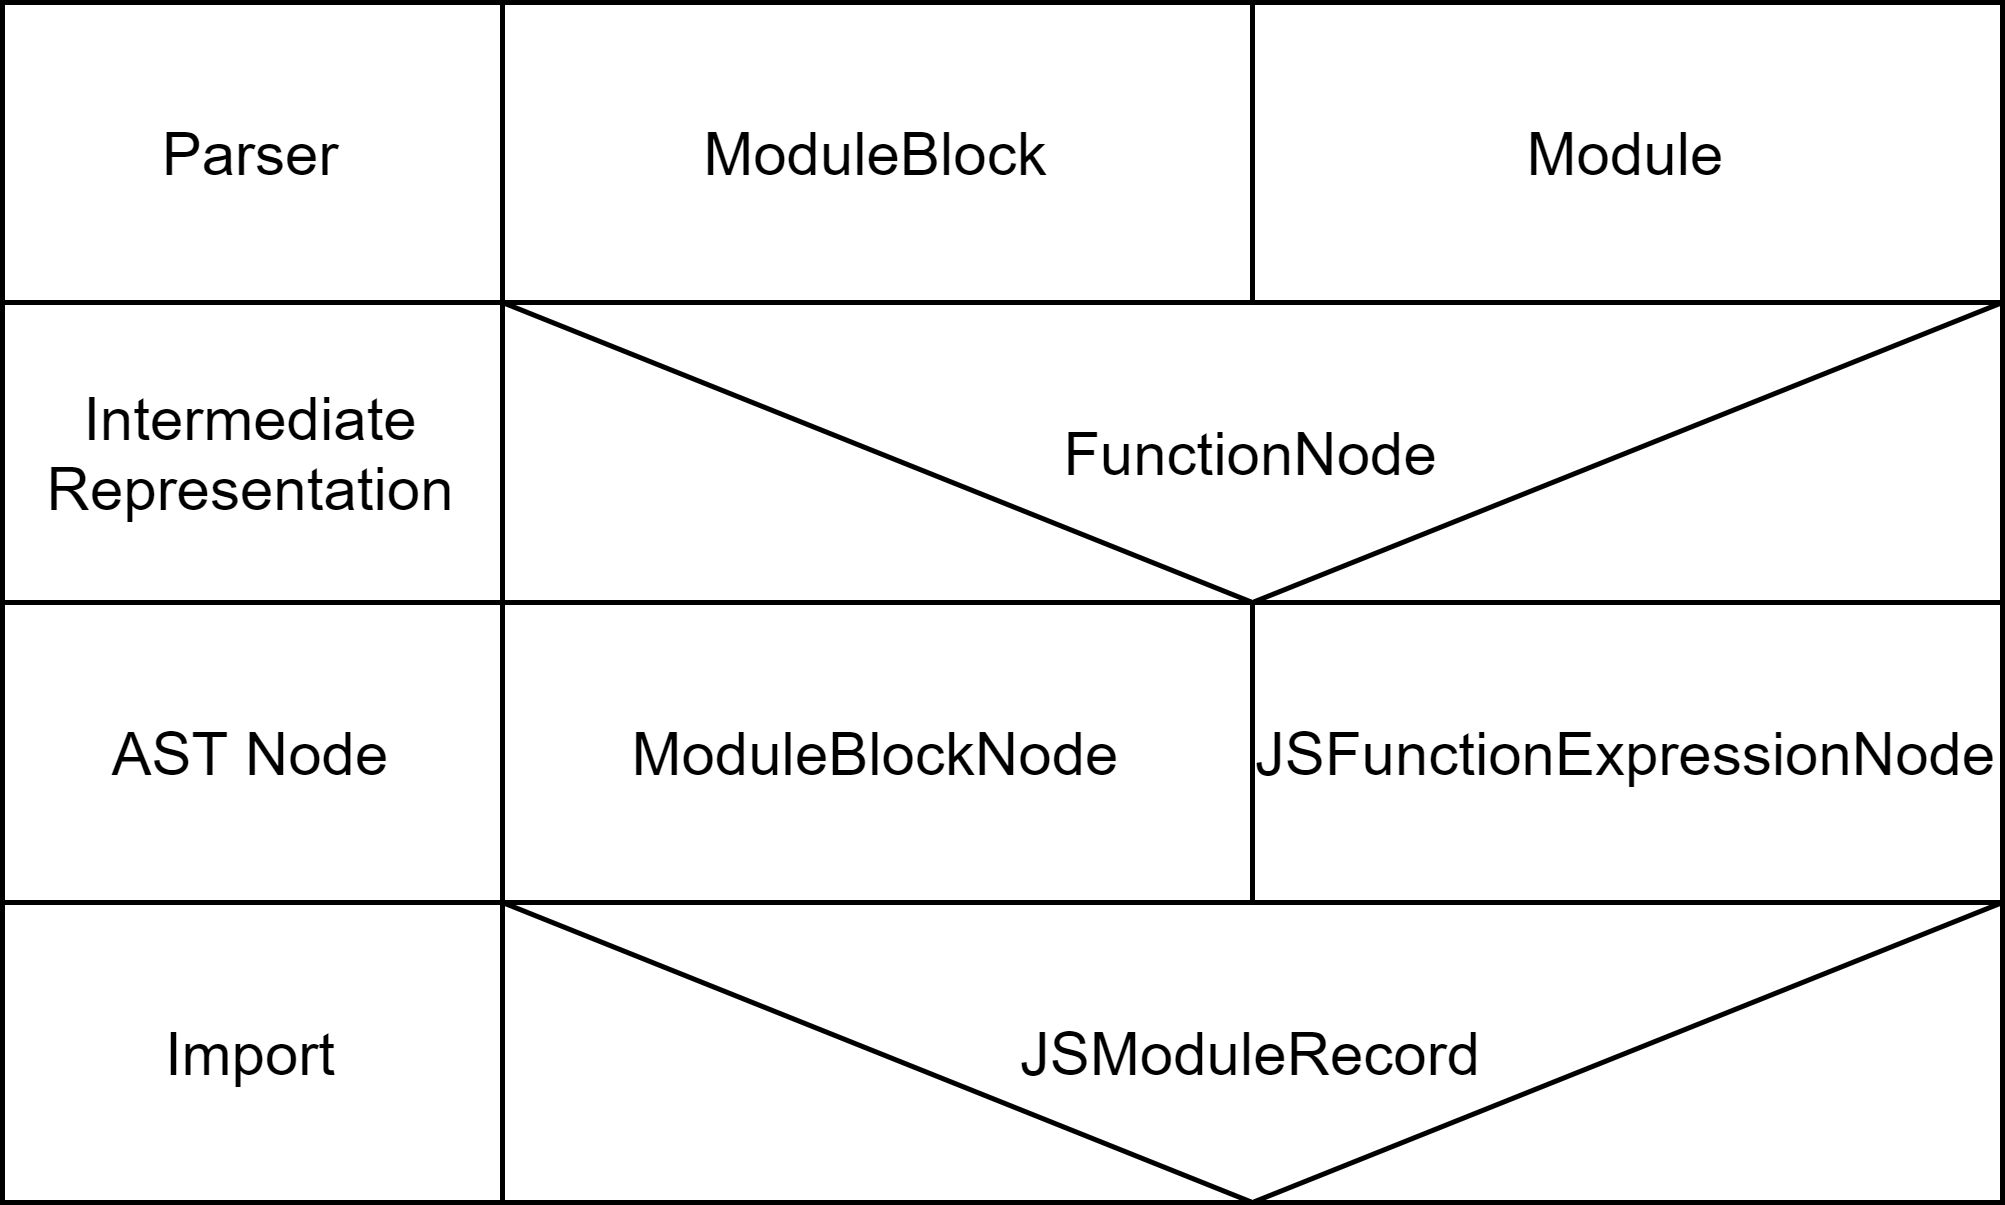
\includegraphics[scale=0.165]{figures/ModuleBlockVSModule.png}
    \caption{Simplified Graal.js translation pipeline of module blocks and modules}
    \label{fig:blockVSmodule}
\end{figure}

\chapter{Evaluation}

The presented module blocks implementation which has been embedded inside the Graal.js project, was evaluated by running the provided tests in the project. Those tests represent the Test262 implementation conformance test suite. \cite{ecmaTest262} Since these tests can't cover module block syntax and semantics additional tests were conducted.

The Test262 suite combines the three ecma standards ECMA-262, ECMAScript Language Specification, ECMA-402, ECMAScript Internationalization API Specification and ECMA-404 the JSON Data Interchange Syntax, also known as ISO/IEC 21778. The suite's test files cover any  behavior stated in these specifications and is comprised of around 30.000 individual test files. \cite{ecmaTest262, ecmaTestSpec} Although the test environment is extensive full coverage cannot be guaranteed. It's certain to say that the suite doesn't yet contain any tests that cover module block functionality. This shifts the topic towards the tests that were designed and conducted in the course of this thesis.

The main orientation for designing tests regarding the module block proposal came from the available basic specification. While it is not finished yet, the parts of the specification that could be implemented can also be tested. First of, the syntactic part of the specification can already pose different testing scenarios.

\begin{figure}[h!]
    \begin{lstlisting}
        var module = 42;
        
        var nextModule = module;
        
        var moduleBlock = module { };
        
        var failingModuleBlock = module
            { };
    \end{lstlisting}
\caption{Module block syntax tests}
\label{fig:testSyntax}
\end{figure}

The first syntactic specialty is the fact that "module", while acting as a keyword in the scope of module blocks, won't be added to the keywords group in ECMAScript. The consequences are random variables being used with "module" as identifier are allowed and line delimiters between "module" and the "\{" are forbidden. Since the ModuleBody part of the module block syntax  is optional an empty module like in line three of figure \ref{fig:testSyntax}. This concludes the three testing cases for the syntax. Next up are tests regarding the prototype and the constructor.

The constructor of module blocks basically doesn't have to exist as it simply should throw a TypeError. The decision during implementation was made that it actually is implemented but when called throws the specified error. Still it doesn't change the expected behavior and thus a simple call to the constructor is made and expects the aforementioned error. Testing the prototype requires more elaborate testing since multiple aspects need to be checked. Those regard especially the prototype property of the module block prototype object itself but also the module block prototype property. The described tests are conducted by source code similar to figure \ref{fig:testCoPro}.

\begin{figure}[h!]
    \begin{lstlisting}
        var constructorModuleBlock = new ModuleBlock(); // TypeError: ModuleBlock is not a constructor
        
        var moduleBlock = module { };
        
        var instanceTest = moduleBlock instanceof ModuleBlock; // true
        
        var moduleBlockPrototype = moduleBlock.prototype; // object
    \end{lstlisting}
    \caption{Module block constructor and prototype tests}
    \label{fig:testCoPro}
\end{figure}

The following tests mainly regard the module blocks interaction with different ECMAScript constructs inside of the module block, in particular the optional syntax part ModuleBody, and its interaction with the dynamic import. The interaction with existing ECMAScript structures is straightforward as all of them have to be used inside a module block as part of the ModuleBody to some extent. The following figure \ref{fig:testGeneral} list some example cases with a simple number variable, a function and an async function.

\begin{figure}[h!]
    \begin{lstlisting}
        var moduleBlock = module { export var x = 42; }; // export number
        
        var moduleBlockFunc = module { export function square(x) {
                return x * x;
            } 
        }; // export function
    
        var moduleBlockAsync = module {
            function resolve() {
                return new Promise(resolve => {
                        resolve('resolved inside module block')
                });
            }
        
            async function asyncCall() {
                return await resolve();
            }
        
            export var resolved = asyncCall(); 
        }; // export promise
    \end{lstlisting}
    \caption{Module block general test example cases}
    \label{fig:testGeneral}
\end{figure}

A particular case that should also be noted as it raised interest during the proposal presentation is the ability to bundle module imports into a module block which was also tested extensively with importing modules in the different possible ways and also importing module blocks. The specialties of module block imports are explained in the next bit.

Module blocks can only be imported dynamically with awaits. Since top level awaits are not supported dynamic imports have to be encapsulated in async functions. Hence imported module block module records are encapsulated in a promise and have to be processed in a then-environment. Figure \ref{fig:testImp} shows the exact syntax needed for importing the module block.

\begin{figure}[h!]
    \begin{lstlisting}
        var test = (async function() {
            var moduleBlock = module { export var x = 42; }; // export number
            
            return await import(moduleBlock);
        })();
        
        test.then( function(module) {
            console.log("Module block x: " + module.x);  // Module block x: 42
        });
    \end{lstlisting}
    \caption{Module block dynamic import test}
    \label{fig:testImp}
\end{figure}

In conclusion adding a new feature into an engine for ECMAScript requires extensive testing. First of the general preexisting test suite Test262 has to be applied to the changed semantics and have to pass. Then all intricacies of the proposal's specification have to be tested. Although the proposal is a rather syntactic one it still introduces semantics which have to be tested. Next up after all internals are checked the interaction with preexisting ECMAScript structures needs to take place which furthers the extensiveness of testing.

\chapter{Future Work}

Future Work on the thesis's matter is tightly tied to progress on the module block proposal. At current state the proposal resides at stage two where neither the specification is finalized nor the details are all cleared. A specific case of this is the hostInitializeModuleBlock-method mentioned in the runtime semantics of the module block specification, as it is merely mentioned but not specified. The work needs to be continued to keep the implementation on par with the specification. Especially as soon as the proposal reaches stage three the final specification is available. Subsequently the implementation has to be adjusted to fit the final version. Furthermore as the proposal progresses official tests will be released and later on embedded into the official Test262 suite. Those tests then have to be applied to the finished implementation. The preceding development description is rather rough, therefore the following paragraphs discuss details on the proposal that are not fixed yet.

A controversial implementation detail up for possible change is the constructor of module blocks. At current development state a constructor call leads to a \texttt{TypeError}. The relevant point for rejecting the ability to create a module block via a constructor is that module blocks would turn into an eval-like structure which is unwanted for as the web community generally rejects the eval-method. Due to security issues this sentiment gained widespread support. On the other hand one can argue that a language's design should be sound and symmetrical. Other structures that were introduced in ECMAScript that share the eval-like constructor discussion do have a working constructor. Thus for reasons of symmetry module blocks should have a constructor as well. The result of the discussion will be visible latest at stage three of the proposal. Right now the simple constructor implementation only throws the error and would have to be fully implemented if a working constructor is introduced in the proposal.

Another feature that might be introduced is an abbreviated form of module blocks. Due to the feature's rather syntactic nature the requirement are parser changes leading then into the same semantics as module blocks. The feature might be included if import-free-single-function module blocks become a frequently recurring pattern. Also not entirely clear is what the import.meta.url of a module block should look like. Although it is save to assume that it's bound to the module's \texttt{import.meta.url} in which it is specified it is frowned upon to be the exact same. A possible setup would be the module's import.meta.url directly followed by something like: "$L\#^+C\#^+$" where the \#s stand for the exact line and column number of the module block. As this is also not fixed yet the implementation has to follow suit as soon as the import.meta.url semantics are fixed.

In short, the implementation cannot be finalized in the scope of the thesis as the proposal hasn't reached stage 4 by then. A lot of details need to be worked on before the proposal can reach stage three. With stage three reached the implementation can be finished as the specification will be finished more or less. The testing in the scope of the thesis has to be adapted to the final implementation and the tests being released before the proposal can reach stage four. Since the implementation is tied closely to the proposal it can only be done as soon as the proposal is completed and adopted by moving to stage 4 which is possible earliest in 2022.

As much as the implementation is bound to the proposal, the testing is bound to the implementation and thus cannot be finalized until the proposal is adopted. The aforementioned features all have to be tested separately. It should also be noted that the performance tests conducted in the scope of the thesis test for module block call's performance loss exclusively, but the performance should also be measured in real-world examples to test general runtime metrics. However, these particular tests should be conducted in a later state of the proposal as a lot of the semantics are not fixed yet. In conclusion, testing should be continued and intensified alongside the implementation and proposal development.


\chapter{Conclusions}

%In the scope of the thesis the ECMAScript TC39 proposal "module blocks" was implemented into the Graal.js project which resides inside the GraalVM ecosystem. The implementation was split into a syntactic and semantic part, with the semantic part being conducted through introducing a new Node according to general Truffle rules and the given proposal specification. The syntactic part was introduced via minor changes in the preexisting Graal.js parser. Testing the implementation consisted of applying the preexisting Test262 official ECMAScript test suite and explicitly for the proposal written unit tests on it. To finish off embedding the proposal a serialization algorithm was written and tested with a proof of concept test via a Worker. Reiterating the fact that the proposal is not finished yet and supposed to undergo changes, it can be said that the base for contributing this stage two proposal to the Graal.js project is laid out.

In the scope of the thesis the ECMAScript TC39 proposal module blocks was implemented into the Graal.js project which resides inside the GraalVM ecosystem. The proposal enhances module usage in ECMAScript and has thus the potential to greatly impact their usage throughout the internet especially by simplifying use of Workers. For this to happen the proposal itself is not enough, at least not in the Graal.js project since code has to be serialized before being sent to another process. The serialization and deserialization is also implemented in order to enhance the practical feasibility. Now, inline JavaScript code can be sent back and forth between processes resulting in lower network footprint as code and results have to be sent but not whole data packages. Another point to keep in mind that early proposal adaptation greatly helps keeping on par with the ECMAScript specification's development but also the rival engines. The implementation passes the preexisting Test262 official ECMAScript test suite and explicitly for the proposal written unit tests on it. In the thesis it was shown that the module block implementation has no performance downside compared to regular code like function calls or modules. This was shown via toy examples and should be matured alongside further implementation and proposal development. Since the proposal is not finished yet the thesis laid the groundwork for implementing the upcoming further developments on the proposal into the Graal.js project.





%%%%%%%%%%%
\begin{singlespace}
	\listoffigures
    \lstlistoflistings
\end{singlespace}


\backmatter

\printbibliography

\appendix

\end{document}
